\section{Geometric measurements and language spectral interventions}\label{app:complete-interventions}
\FloatBarrier
\subsection{Checkpoints, controls and reference models}
The intervention study covers 108 checkpoints selected by mean development accuracy within each model/method/capacity, with 22 interventions or controls per checkpoint. Llama HRA uses the extended-grid selections in Appendix~\ref{app:hra-extension}. All edits use the same GSM8K development and general-text banks. The tables below extend the largest-capacity main figures to all capacities and selected LRs.

Task and NLL changes use the trained model as reference. Value-restoration controls compare against reconstruction, while component sufficiency and factorial analyses use full value restoration. Forgetting recovery is the fraction of the trained model's NLL increase recovered by an edit, computed within each checkpoint before seed averaging.

Edits jointly cover all adapted matrices. SVD computations use FP32, followed by BF16 storage and evaluation. The dominant, intermediate and trailing component groups divide the pretrained spectrum into approximate thirds, with boundaries adjusted to nearby spectral gaps. Plots label these groups top, middle and tail.

For the collection $\mathcal M$ of adapted matrices, the normalized displacements are
\begin{equation*}
 d_W^2=\frac{\sum_{M\in\mathcal M}\left\|\bm W_{*,M}-\bm W_{0,M}\right\|_{\mathrm F}^2}{\sum_{M\in\mathcal M}\left\|\bm W_{0,M}\right\|_{\mathrm F}^2},\qquad
 d_S^2=\frac{\sum_{M\in\mathcal M}\left\|\bm s_{*,M}-\bm s_{0,M}\right\|_2^2}{\sum_{M\in\mathcal M}\left\|\bm s_{0,M}\right\|_2^2}.
\end{equation*}

Each checkpoint pools all 196 Qwen or 224 Llama adapted matrices (80 for the FLUX results in Appendix~\ref{app:flux22}), weighting their contributions through the squared norms.

\begin{table}[!htbp]
\caption{Qwen2.5-7B spectral displacement at every selected capacity and LR.}
\label{tab:peft-spectrum-qwen}
\begin{center}
\setlength{\tabcolsep}{3pt}
\begin{tabular*}{\linewidth}{@{\extracolsep{\fill}}lrrrrr@{}}\toprule
Method & Capacity & LR & $100d_W$ & $100d_S$ & $100d_S/d_W$\\\midrule
\textcolor{LoRAColor}{LoRA} & 7 & $1\times10^{-3}$ & $\result{rev_qwen_lora_7_trained_d_W_mean}_{\pm \result{rev_qwen_lora_7_trained_d_W_sd}}$ & $\result{rev_qwen_lora_7_trained_d_S_mean}_{\pm \result{rev_qwen_lora_7_trained_d_S_sd}}$ & $\result{rev_qwen_lora_7_trained_ratio_mean}_{\pm \result{rev_qwen_lora_7_trained_ratio_sd}}$\\
\textcolor{LoRAColor}{LoRA} & 14 & $1\times10^{-5}$ & $\result{rev_qwen_lora_14_trained_d_W_mean}_{\pm \result{rev_qwen_lora_14_trained_d_W_sd}}$ & $\result{rev_qwen_lora_14_trained_d_S_mean}_{\pm \result{rev_qwen_lora_14_trained_d_S_sd}}$ & $\result{rev_qwen_lora_14_trained_ratio_mean}_{\pm \result{rev_qwen_lora_14_trained_ratio_sd}}$\\
\textcolor{LoRAColor}{LoRA} & 28 & $3\times10^{-5}$ & $\result{rev_qwen_lora_28_trained_d_W_mean}_{\pm \result{rev_qwen_lora_28_trained_d_W_sd}}$ & $\result{rev_qwen_lora_28_trained_d_S_mean}_{\pm \result{rev_qwen_lora_28_trained_d_S_sd}}$ & $\result{rev_qwen_lora_28_trained_ratio_mean}_{\pm \result{rev_qwen_lora_28_trained_ratio_sd}}$\\
\addlinespace[2pt]
\textcolor{OFTColor}{OFT} & 32 & $3\times10^{-4}$ & $\result{rev_qwen_oft_32_trained_d_W_mean}_{\pm \result{rev_qwen_oft_32_trained_d_W_sd}}$ & $\result{rev_qwen_oft_32_trained_d_S_mean}_{\pm \result{rev_qwen_oft_32_trained_d_S_sd}}$ & $\result{rev_qwen_oft_32_trained_ratio_mean}_{\pm \result{rev_qwen_oft_32_trained_ratio_sd}}$\\
\textcolor{OFTColor}{OFT} & 64 & $3\times10^{-4}$ & $\result{rev_qwen_oft_64_trained_d_W_mean}_{\pm \result{rev_qwen_oft_64_trained_d_W_sd}}$ & $\result{rev_qwen_oft_64_trained_d_S_mean}_{\pm \result{rev_qwen_oft_64_trained_d_S_sd}}$ & $\result{rev_qwen_oft_64_trained_ratio_mean}_{\pm \result{rev_qwen_oft_64_trained_ratio_sd}}$\\
\textcolor{OFTColor}{OFT} & 128 & $1\times10^{-4}$ & $\result{rev_qwen_oft_128_trained_d_W_mean}_{\pm \result{rev_qwen_oft_128_trained_d_W_sd}}$ & $\result{rev_qwen_oft_128_trained_d_S_mean}_{\pm \result{rev_qwen_oft_128_trained_d_S_sd}}$ & $\result{rev_qwen_oft_128_trained_ratio_mean}_{\pm \result{rev_qwen_oft_128_trained_ratio_sd}}$\\
\addlinespace[2pt]
\textcolor{DoRAColor}{DoRA} & 7 & $3\times10^{-4}$ & $\result{rev_qwen_dora_7_trained_d_W_mean}_{\pm \result{rev_qwen_dora_7_trained_d_W_sd}}$ & $\result{rev_qwen_dora_7_trained_d_S_mean}_{\pm \result{rev_qwen_dora_7_trained_d_S_sd}}$ & $\result{rev_qwen_dora_7_trained_ratio_mean}_{\pm \result{rev_qwen_dora_7_trained_ratio_sd}}$\\
\textcolor{DoRAColor}{DoRA} & 14 & $3\times10^{-4}$ & $\result{rev_qwen_dora_14_trained_d_W_mean}_{\pm \result{rev_qwen_dora_14_trained_d_W_sd}}$ & $\result{rev_qwen_dora_14_trained_d_S_mean}_{\pm \result{rev_qwen_dora_14_trained_d_S_sd}}$ & $\result{rev_qwen_dora_14_trained_ratio_mean}_{\pm \result{rev_qwen_dora_14_trained_ratio_sd}}$\\
\textcolor{DoRAColor}{DoRA} & 28 & $1\times10^{-4}$ & $\result{rev_qwen_dora_28_trained_d_W_mean}_{\pm \result{rev_qwen_dora_28_trained_d_W_sd}}$ & $\result{rev_qwen_dora_28_trained_d_S_mean}_{\pm \result{rev_qwen_dora_28_trained_d_S_sd}}$ & $\result{rev_qwen_dora_28_trained_ratio_mean}_{\pm \result{rev_qwen_dora_28_trained_ratio_sd}}$\\
\addlinespace[2pt]
\textcolor{PiSSAColor}{PiSSA} & 7 & $3\times10^{-5}$ & $\result{rev_qwen_pissa_7_trained_d_W_mean}_{\pm \result{rev_qwen_pissa_7_trained_d_W_sd}}$ & $\result{rev_qwen_pissa_7_trained_d_S_mean}_{\pm \result{rev_qwen_pissa_7_trained_d_S_sd}}$ & $\result{rev_qwen_pissa_7_trained_ratio_mean}_{\pm \result{rev_qwen_pissa_7_trained_ratio_sd}}$\\
\textcolor{PiSSAColor}{PiSSA} & 14 & $3\times10^{-5}$ & $\result{rev_qwen_pissa_14_trained_d_W_mean}_{\pm \result{rev_qwen_pissa_14_trained_d_W_sd}}$ & $\result{rev_qwen_pissa_14_trained_d_S_mean}_{\pm \result{rev_qwen_pissa_14_trained_d_S_sd}}$ & $\result{rev_qwen_pissa_14_trained_ratio_mean}_{\pm \result{rev_qwen_pissa_14_trained_ratio_sd}}$\\
\textcolor{PiSSAColor}{PiSSA} & 28 & $3\times10^{-5}$ & $\result{rev_qwen_pissa_28_trained_d_W_mean}_{\pm \result{rev_qwen_pissa_28_trained_d_W_sd}}$ & $\result{rev_qwen_pissa_28_trained_d_S_mean}_{\pm \result{rev_qwen_pissa_28_trained_d_S_sd}}$ & $\result{rev_qwen_pissa_28_trained_ratio_mean}_{\pm \result{rev_qwen_pissa_28_trained_ratio_sd}}$\\
\addlinespace[2pt]
\textcolor{MiLoRAColor}{MiLoRA} & 7 & $1\times10^{-5}$ & $\result{rev_qwen_milora_7_trained_d_W_mean}_{\pm \result{rev_qwen_milora_7_trained_d_W_sd}}$ & $\result{rev_qwen_milora_7_trained_d_S_mean}_{\pm \result{rev_qwen_milora_7_trained_d_S_sd}}$ & $\result{rev_qwen_milora_7_trained_ratio_mean}_{\pm \result{rev_qwen_milora_7_trained_ratio_sd}}$\\
\textcolor{MiLoRAColor}{MiLoRA} & 14 & $1\times10^{-5}$ & $\result{rev_qwen_milora_14_trained_d_W_mean}_{\pm \result{rev_qwen_milora_14_trained_d_W_sd}}$ & $\result{rev_qwen_milora_14_trained_d_S_mean}_{\pm \result{rev_qwen_milora_14_trained_d_S_sd}}$ & $\result{rev_qwen_milora_14_trained_ratio_mean}_{\pm \result{rev_qwen_milora_14_trained_ratio_sd}}$\\
\textcolor{MiLoRAColor}{MiLoRA} & 28 & $3\times10^{-5}$ & $\result{rev_qwen_milora_28_trained_d_W_mean}_{\pm \result{rev_qwen_milora_28_trained_d_W_sd}}$ & $\result{rev_qwen_milora_28_trained_d_S_mean}_{\pm \result{rev_qwen_milora_28_trained_d_S_sd}}$ & $\result{rev_qwen_milora_28_trained_ratio_mean}_{\pm \result{rev_qwen_milora_28_trained_ratio_sd}}$\\
\addlinespace[2pt]
\textcolor{HRAColor}{HRA} & 16 & $1\times10^{-4}$ & $\result{rev_qwen_hra_16_trained_d_W_mean}_{\pm \result{rev_qwen_hra_16_trained_d_W_sd}}$ & $\result{rev_qwen_hra_16_trained_d_S_mean}_{\pm \result{rev_qwen_hra_16_trained_d_S_sd}}$ & $\result{rev_qwen_hra_16_trained_ratio_mean}_{\pm \result{rev_qwen_hra_16_trained_ratio_sd}}$\\
\textcolor{HRAColor}{HRA} & 32 & $1\times10^{-4}$ & $\result{rev_qwen_hra_32_trained_d_W_mean}_{\pm \result{rev_qwen_hra_32_trained_d_W_sd}}$ & $\result{rev_qwen_hra_32_trained_d_S_mean}_{\pm \result{rev_qwen_hra_32_trained_d_S_sd}}$ & $\result{rev_qwen_hra_32_trained_ratio_mean}_{\pm \result{rev_qwen_hra_32_trained_ratio_sd}}$\\
\textcolor{HRAColor}{HRA} & 64 & $1\times10^{-5}$ & $\result{rev_qwen_hra_64_trained_d_W_mean}_{\pm \result{rev_qwen_hra_64_trained_d_W_sd}}$ & $\result{rev_qwen_hra_64_trained_d_S_mean}_{\pm \result{rev_qwen_hra_64_trained_d_S_sd}}$ & $\result{rev_qwen_hra_64_trained_ratio_mean}_{\pm \result{rev_qwen_hra_64_trained_ratio_sd}}$\\
\bottomrule\end{tabular*}
\end{center}
\end{table}
\FloatBarrier
\begin{table}[!htbp]
\caption{Qwen2.5-7B singular-value restoration and reconstruction controls, with accuracy in percent.}
\label{tab:peft-restoration-qwen}
\begin{center}
\setlength{\tabcolsep}{3pt}
\begin{tabular*}{\linewidth}{@{\extracolsep{\fill}}lrrrrrr@{}}\toprule
Method & Capacity & LR & Trained acc. & Rebuilt acc. & Restored acc. & $\Delta$NLL vs. rebuilt\\\midrule
\textcolor{LoRAColor}{LoRA} & 7 & $1\times10^{-3}$ & $\result{rev_qwen_lora_7_trained_accuracy_mean}_{\pm \result{rev_qwen_lora_7_trained_accuracy_sd}}$ & $\result{rev_qwen_lora_7_reconstruct_accuracy_mean}_{\pm \result{rev_qwen_lora_7_reconstruct_accuracy_sd}}$ & $\result{rev_qwen_lora_7_restore_accuracy_mean}_{\pm \result{rev_qwen_lora_7_restore_accuracy_sd}}$ & $\result{rev_qwen_lora_7_restore_nll_vs_reconstruct_mean}_{\pm \result{rev_qwen_lora_7_restore_nll_vs_reconstruct_sd}}$\\
\textcolor{LoRAColor}{LoRA} & 14 & $1\times10^{-5}$ & $\result{rev_qwen_lora_14_trained_accuracy_mean}_{\pm \result{rev_qwen_lora_14_trained_accuracy_sd}}$ & $\result{rev_qwen_lora_14_reconstruct_accuracy_mean}_{\pm \result{rev_qwen_lora_14_reconstruct_accuracy_sd}}$ & $\result{rev_qwen_lora_14_restore_accuracy_mean}_{\pm \result{rev_qwen_lora_14_restore_accuracy_sd}}$ & $\result{rev_qwen_lora_14_restore_nll_vs_reconstruct_mean}_{\pm \result{rev_qwen_lora_14_restore_nll_vs_reconstruct_sd}}$\\
\textcolor{LoRAColor}{LoRA} & 28 & $3\times10^{-5}$ & $\result{rev_qwen_lora_28_trained_accuracy_mean}_{\pm \result{rev_qwen_lora_28_trained_accuracy_sd}}$ & $\result{rev_qwen_lora_28_reconstruct_accuracy_mean}_{\pm \result{rev_qwen_lora_28_reconstruct_accuracy_sd}}$ & $\result{rev_qwen_lora_28_restore_accuracy_mean}_{\pm \result{rev_qwen_lora_28_restore_accuracy_sd}}$ & $\result{rev_qwen_lora_28_restore_nll_vs_reconstruct_mean}_{\pm \result{rev_qwen_lora_28_restore_nll_vs_reconstruct_sd}}$\\
\addlinespace[2pt]
\textcolor{OFTColor}{OFT} & 32 & $3\times10^{-4}$ & $\result{rev_qwen_oft_32_trained_accuracy_mean}_{\pm \result{rev_qwen_oft_32_trained_accuracy_sd}}$ & $\result{rev_qwen_oft_32_reconstruct_accuracy_mean}_{\pm \result{rev_qwen_oft_32_reconstruct_accuracy_sd}}$ & $\result{rev_qwen_oft_32_restore_accuracy_mean}_{\pm \result{rev_qwen_oft_32_restore_accuracy_sd}}$ & $\result{rev_qwen_oft_32_restore_nll_vs_reconstruct_mean}_{\pm \result{rev_qwen_oft_32_restore_nll_vs_reconstruct_sd}}$\\
\textcolor{OFTColor}{OFT} & 64 & $3\times10^{-4}$ & $\result{rev_qwen_oft_64_trained_accuracy_mean}_{\pm \result{rev_qwen_oft_64_trained_accuracy_sd}}$ & $\result{rev_qwen_oft_64_reconstruct_accuracy_mean}_{\pm \result{rev_qwen_oft_64_reconstruct_accuracy_sd}}$ & $\result{rev_qwen_oft_64_restore_accuracy_mean}_{\pm \result{rev_qwen_oft_64_restore_accuracy_sd}}$ & $\result{rev_qwen_oft_64_restore_nll_vs_reconstruct_mean}_{\pm \result{rev_qwen_oft_64_restore_nll_vs_reconstruct_sd}}$\\
\textcolor{OFTColor}{OFT} & 128 & $1\times10^{-4}$ & $\result{rev_qwen_oft_128_trained_accuracy_mean}_{\pm \result{rev_qwen_oft_128_trained_accuracy_sd}}$ & $\result{rev_qwen_oft_128_reconstruct_accuracy_mean}_{\pm \result{rev_qwen_oft_128_reconstruct_accuracy_sd}}$ & $\result{rev_qwen_oft_128_restore_accuracy_mean}_{\pm \result{rev_qwen_oft_128_restore_accuracy_sd}}$ & $\result{rev_qwen_oft_128_restore_nll_vs_reconstruct_mean}_{\pm \result{rev_qwen_oft_128_restore_nll_vs_reconstruct_sd}}$\\
\addlinespace[2pt]
\textcolor{DoRAColor}{DoRA} & 7 & $3\times10^{-4}$ & $\result{rev_qwen_dora_7_trained_accuracy_mean}_{\pm \result{rev_qwen_dora_7_trained_accuracy_sd}}$ & $\result{rev_qwen_dora_7_reconstruct_accuracy_mean}_{\pm \result{rev_qwen_dora_7_reconstruct_accuracy_sd}}$ & $\result{rev_qwen_dora_7_restore_accuracy_mean}_{\pm \result{rev_qwen_dora_7_restore_accuracy_sd}}$ & $\result{rev_qwen_dora_7_restore_nll_vs_reconstruct_mean}_{\pm \result{rev_qwen_dora_7_restore_nll_vs_reconstruct_sd}}$\\
\textcolor{DoRAColor}{DoRA} & 14 & $3\times10^{-4}$ & $\result{rev_qwen_dora_14_trained_accuracy_mean}_{\pm \result{rev_qwen_dora_14_trained_accuracy_sd}}$ & $\result{rev_qwen_dora_14_reconstruct_accuracy_mean}_{\pm \result{rev_qwen_dora_14_reconstruct_accuracy_sd}}$ & $\result{rev_qwen_dora_14_restore_accuracy_mean}_{\pm \result{rev_qwen_dora_14_restore_accuracy_sd}}$ & $\result{rev_qwen_dora_14_restore_nll_vs_reconstruct_mean}_{\pm \result{rev_qwen_dora_14_restore_nll_vs_reconstruct_sd}}$\\
\textcolor{DoRAColor}{DoRA} & 28 & $1\times10^{-4}$ & $\result{rev_qwen_dora_28_trained_accuracy_mean}_{\pm \result{rev_qwen_dora_28_trained_accuracy_sd}}$ & $\result{rev_qwen_dora_28_reconstruct_accuracy_mean}_{\pm \result{rev_qwen_dora_28_reconstruct_accuracy_sd}}$ & $\result{rev_qwen_dora_28_restore_accuracy_mean}_{\pm \result{rev_qwen_dora_28_restore_accuracy_sd}}$ & $\result{rev_qwen_dora_28_restore_nll_vs_reconstruct_mean}_{\pm \result{rev_qwen_dora_28_restore_nll_vs_reconstruct_sd}}$\\
\addlinespace[2pt]
\textcolor{PiSSAColor}{PiSSA} & 7 & $3\times10^{-5}$ & $\result{rev_qwen_pissa_7_trained_accuracy_mean}_{\pm \result{rev_qwen_pissa_7_trained_accuracy_sd}}$ & $\result{rev_qwen_pissa_7_reconstruct_accuracy_mean}_{\pm \result{rev_qwen_pissa_7_reconstruct_accuracy_sd}}$ & $\result{rev_qwen_pissa_7_restore_accuracy_mean}_{\pm \result{rev_qwen_pissa_7_restore_accuracy_sd}}$ & $\result{rev_qwen_pissa_7_restore_nll_vs_reconstruct_mean}_{\pm \result{rev_qwen_pissa_7_restore_nll_vs_reconstruct_sd}}$\\
\textcolor{PiSSAColor}{PiSSA} & 14 & $3\times10^{-5}$ & $\result{rev_qwen_pissa_14_trained_accuracy_mean}_{\pm \result{rev_qwen_pissa_14_trained_accuracy_sd}}$ & $\result{rev_qwen_pissa_14_reconstruct_accuracy_mean}_{\pm \result{rev_qwen_pissa_14_reconstruct_accuracy_sd}}$ & $\result{rev_qwen_pissa_14_restore_accuracy_mean}_{\pm \result{rev_qwen_pissa_14_restore_accuracy_sd}}$ & $\result{rev_qwen_pissa_14_restore_nll_vs_reconstruct_mean}_{\pm \result{rev_qwen_pissa_14_restore_nll_vs_reconstruct_sd}}$\\
\textcolor{PiSSAColor}{PiSSA} & 28 & $3\times10^{-5}$ & $\result{rev_qwen_pissa_28_trained_accuracy_mean}_{\pm \result{rev_qwen_pissa_28_trained_accuracy_sd}}$ & $\result{rev_qwen_pissa_28_reconstruct_accuracy_mean}_{\pm \result{rev_qwen_pissa_28_reconstruct_accuracy_sd}}$ & $\result{rev_qwen_pissa_28_restore_accuracy_mean}_{\pm \result{rev_qwen_pissa_28_restore_accuracy_sd}}$ & $\result{rev_qwen_pissa_28_restore_nll_vs_reconstruct_mean}_{\pm \result{rev_qwen_pissa_28_restore_nll_vs_reconstruct_sd}}$\\
\addlinespace[2pt]
\textcolor{MiLoRAColor}{MiLoRA} & 7 & $1\times10^{-5}$ & $\result{rev_qwen_milora_7_trained_accuracy_mean}_{\pm \result{rev_qwen_milora_7_trained_accuracy_sd}}$ & $\result{rev_qwen_milora_7_reconstruct_accuracy_mean}_{\pm \result{rev_qwen_milora_7_reconstruct_accuracy_sd}}$ & $\result{rev_qwen_milora_7_restore_accuracy_mean}_{\pm \result{rev_qwen_milora_7_restore_accuracy_sd}}$ & $\result{rev_qwen_milora_7_restore_nll_vs_reconstruct_mean}_{\pm \result{rev_qwen_milora_7_restore_nll_vs_reconstruct_sd}}$\\
\textcolor{MiLoRAColor}{MiLoRA} & 14 & $1\times10^{-5}$ & $\result{rev_qwen_milora_14_trained_accuracy_mean}_{\pm \result{rev_qwen_milora_14_trained_accuracy_sd}}$ & $\result{rev_qwen_milora_14_reconstruct_accuracy_mean}_{\pm \result{rev_qwen_milora_14_reconstruct_accuracy_sd}}$ & $\result{rev_qwen_milora_14_restore_accuracy_mean}_{\pm \result{rev_qwen_milora_14_restore_accuracy_sd}}$ & $\result{rev_qwen_milora_14_restore_nll_vs_reconstruct_mean}_{\pm \result{rev_qwen_milora_14_restore_nll_vs_reconstruct_sd}}$\\
\textcolor{MiLoRAColor}{MiLoRA} & 28 & $3\times10^{-5}$ & $\result{rev_qwen_milora_28_trained_accuracy_mean}_{\pm \result{rev_qwen_milora_28_trained_accuracy_sd}}$ & $\result{rev_qwen_milora_28_reconstruct_accuracy_mean}_{\pm \result{rev_qwen_milora_28_reconstruct_accuracy_sd}}$ & $\result{rev_qwen_milora_28_restore_accuracy_mean}_{\pm \result{rev_qwen_milora_28_restore_accuracy_sd}}$ & $\result{rev_qwen_milora_28_restore_nll_vs_reconstruct_mean}_{\pm \result{rev_qwen_milora_28_restore_nll_vs_reconstruct_sd}}$\\
\addlinespace[2pt]
\textcolor{HRAColor}{HRA} & 16 & $1\times10^{-4}$ & $\result{rev_qwen_hra_16_trained_accuracy_mean}_{\pm \result{rev_qwen_hra_16_trained_accuracy_sd}}$ & $\result{rev_qwen_hra_16_reconstruct_accuracy_mean}_{\pm \result{rev_qwen_hra_16_reconstruct_accuracy_sd}}$ & $\result{rev_qwen_hra_16_restore_accuracy_mean}_{\pm \result{rev_qwen_hra_16_restore_accuracy_sd}}$ & $\result{rev_qwen_hra_16_restore_nll_vs_reconstruct_mean}_{\pm \result{rev_qwen_hra_16_restore_nll_vs_reconstruct_sd}}$\\
\textcolor{HRAColor}{HRA} & 32 & $1\times10^{-4}$ & $\result{rev_qwen_hra_32_trained_accuracy_mean}_{\pm \result{rev_qwen_hra_32_trained_accuracy_sd}}$ & $\result{rev_qwen_hra_32_reconstruct_accuracy_mean}_{\pm \result{rev_qwen_hra_32_reconstruct_accuracy_sd}}$ & $\result{rev_qwen_hra_32_restore_accuracy_mean}_{\pm \result{rev_qwen_hra_32_restore_accuracy_sd}}$ & $\result{rev_qwen_hra_32_restore_nll_vs_reconstruct_mean}_{\pm \result{rev_qwen_hra_32_restore_nll_vs_reconstruct_sd}}$\\
\textcolor{HRAColor}{HRA} & 64 & $1\times10^{-5}$ & $\result{rev_qwen_hra_64_trained_accuracy_mean}_{\pm \result{rev_qwen_hra_64_trained_accuracy_sd}}$ & $\result{rev_qwen_hra_64_reconstruct_accuracy_mean}_{\pm \result{rev_qwen_hra_64_reconstruct_accuracy_sd}}$ & $\result{rev_qwen_hra_64_restore_accuracy_mean}_{\pm \result{rev_qwen_hra_64_restore_accuracy_sd}}$ & $\result{rev_qwen_hra_64_restore_nll_vs_reconstruct_mean}_{\pm \result{rev_qwen_hra_64_restore_nll_vs_reconstruct_sd}}$\\
\bottomrule\end{tabular*}
\end{center}
\end{table}
\FloatBarrier
\begin{table}[!htbp]
\caption{Qwen2.5-7B component-restoration effects relative to the trained model, with accuracy changes in percentage points.}
\label{tab:peft-bands-qwen}
\begin{center}
\setlength{\tabcolsep}{3pt}
\begin{tabular*}{\linewidth}{@{\extracolsep{\fill}}lrrrrrr@{}}\toprule
Method & Capacity & LR & Top $\Delta$acc. & Middle $\Delta$acc. & Tail $\Delta$acc. & Top $\Delta$NLL\\\midrule
\textcolor{LoRAColor}{LoRA} & 7 & $1\times10^{-3}$ & $\result{rev_qwen_lora_7_rotation_band_restore_top_accuracy_change_mean}_{\pm \result{rev_qwen_lora_7_rotation_band_restore_top_accuracy_change_sd}}$ & $\result{rev_qwen_lora_7_rotation_band_restore_mid_accuracy_change_mean}_{\pm \result{rev_qwen_lora_7_rotation_band_restore_mid_accuracy_change_sd}}$ & $\result{rev_qwen_lora_7_rotation_band_restore_bottom_accuracy_change_mean}_{\pm \result{rev_qwen_lora_7_rotation_band_restore_bottom_accuracy_change_sd}}$ & $\result{rev_qwen_lora_7_rotation_band_restore_top_nll_change_mean}_{\pm \result{rev_qwen_lora_7_rotation_band_restore_top_nll_change_sd}}$\\
\textcolor{LoRAColor}{LoRA} & 14 & $1\times10^{-5}$ & $\result{rev_qwen_lora_14_rotation_band_restore_top_accuracy_change_mean}_{\pm \result{rev_qwen_lora_14_rotation_band_restore_top_accuracy_change_sd}}$ & $\result{rev_qwen_lora_14_rotation_band_restore_mid_accuracy_change_mean}_{\pm \result{rev_qwen_lora_14_rotation_band_restore_mid_accuracy_change_sd}}$ & $\result{rev_qwen_lora_14_rotation_band_restore_bottom_accuracy_change_mean}_{\pm \result{rev_qwen_lora_14_rotation_band_restore_bottom_accuracy_change_sd}}$ & $\result{rev_qwen_lora_14_rotation_band_restore_top_nll_change_mean}_{\pm \result{rev_qwen_lora_14_rotation_band_restore_top_nll_change_sd}}$\\
\textcolor{LoRAColor}{LoRA} & 28 & $3\times10^{-5}$ & $\result{rev_qwen_lora_28_rotation_band_restore_top_accuracy_change_mean}_{\pm \result{rev_qwen_lora_28_rotation_band_restore_top_accuracy_change_sd}}$ & $\result{rev_qwen_lora_28_rotation_band_restore_mid_accuracy_change_mean}_{\pm \result{rev_qwen_lora_28_rotation_band_restore_mid_accuracy_change_sd}}$ & $\result{rev_qwen_lora_28_rotation_band_restore_bottom_accuracy_change_mean}_{\pm \result{rev_qwen_lora_28_rotation_band_restore_bottom_accuracy_change_sd}}$ & $\result{rev_qwen_lora_28_rotation_band_restore_top_nll_change_mean}_{\pm \result{rev_qwen_lora_28_rotation_band_restore_top_nll_change_sd}}$\\
\addlinespace[2pt]
\textcolor{OFTColor}{OFT} & 32 & $3\times10^{-4}$ & $\result{rev_qwen_oft_32_rotation_band_restore_top_accuracy_change_mean}_{\pm \result{rev_qwen_oft_32_rotation_band_restore_top_accuracy_change_sd}}$ & $\result{rev_qwen_oft_32_rotation_band_restore_mid_accuracy_change_mean}_{\pm \result{rev_qwen_oft_32_rotation_band_restore_mid_accuracy_change_sd}}$ & $\result{rev_qwen_oft_32_rotation_band_restore_bottom_accuracy_change_mean}_{\pm \result{rev_qwen_oft_32_rotation_band_restore_bottom_accuracy_change_sd}}$ & $\result{rev_qwen_oft_32_rotation_band_restore_top_nll_change_mean}_{\pm \result{rev_qwen_oft_32_rotation_band_restore_top_nll_change_sd}}$\\
\textcolor{OFTColor}{OFT} & 64 & $3\times10^{-4}$ & $\result{rev_qwen_oft_64_rotation_band_restore_top_accuracy_change_mean}_{\pm \result{rev_qwen_oft_64_rotation_band_restore_top_accuracy_change_sd}}$ & $\result{rev_qwen_oft_64_rotation_band_restore_mid_accuracy_change_mean}_{\pm \result{rev_qwen_oft_64_rotation_band_restore_mid_accuracy_change_sd}}$ & $\result{rev_qwen_oft_64_rotation_band_restore_bottom_accuracy_change_mean}_{\pm \result{rev_qwen_oft_64_rotation_band_restore_bottom_accuracy_change_sd}}$ & $\result{rev_qwen_oft_64_rotation_band_restore_top_nll_change_mean}_{\pm \result{rev_qwen_oft_64_rotation_band_restore_top_nll_change_sd}}$\\
\textcolor{OFTColor}{OFT} & 128 & $1\times10^{-4}$ & $\result{rev_qwen_oft_128_rotation_band_restore_top_accuracy_change_mean}_{\pm \result{rev_qwen_oft_128_rotation_band_restore_top_accuracy_change_sd}}$ & $\result{rev_qwen_oft_128_rotation_band_restore_mid_accuracy_change_mean}_{\pm \result{rev_qwen_oft_128_rotation_band_restore_mid_accuracy_change_sd}}$ & $\result{rev_qwen_oft_128_rotation_band_restore_bottom_accuracy_change_mean}_{\pm \result{rev_qwen_oft_128_rotation_band_restore_bottom_accuracy_change_sd}}$ & $\result{rev_qwen_oft_128_rotation_band_restore_top_nll_change_mean}_{\pm \result{rev_qwen_oft_128_rotation_band_restore_top_nll_change_sd}}$\\
\addlinespace[2pt]
\textcolor{DoRAColor}{DoRA} & 7 & $3\times10^{-4}$ & $\result{rev_qwen_dora_7_rotation_band_restore_top_accuracy_change_mean}_{\pm \result{rev_qwen_dora_7_rotation_band_restore_top_accuracy_change_sd}}$ & $\result{rev_qwen_dora_7_rotation_band_restore_mid_accuracy_change_mean}_{\pm \result{rev_qwen_dora_7_rotation_band_restore_mid_accuracy_change_sd}}$ & $\result{rev_qwen_dora_7_rotation_band_restore_bottom_accuracy_change_mean}_{\pm \result{rev_qwen_dora_7_rotation_band_restore_bottom_accuracy_change_sd}}$ & $\result{rev_qwen_dora_7_rotation_band_restore_top_nll_change_mean}_{\pm \result{rev_qwen_dora_7_rotation_band_restore_top_nll_change_sd}}$\\
\textcolor{DoRAColor}{DoRA} & 14 & $3\times10^{-4}$ & $\result{rev_qwen_dora_14_rotation_band_restore_top_accuracy_change_mean}_{\pm \result{rev_qwen_dora_14_rotation_band_restore_top_accuracy_change_sd}}$ & $\result{rev_qwen_dora_14_rotation_band_restore_mid_accuracy_change_mean}_{\pm \result{rev_qwen_dora_14_rotation_band_restore_mid_accuracy_change_sd}}$ & $\result{rev_qwen_dora_14_rotation_band_restore_bottom_accuracy_change_mean}_{\pm \result{rev_qwen_dora_14_rotation_band_restore_bottom_accuracy_change_sd}}$ & $\result{rev_qwen_dora_14_rotation_band_restore_top_nll_change_mean}_{\pm \result{rev_qwen_dora_14_rotation_band_restore_top_nll_change_sd}}$\\
\textcolor{DoRAColor}{DoRA} & 28 & $1\times10^{-4}$ & $\result{rev_qwen_dora_28_rotation_band_restore_top_accuracy_change_mean}_{\pm \result{rev_qwen_dora_28_rotation_band_restore_top_accuracy_change_sd}}$ & $\result{rev_qwen_dora_28_rotation_band_restore_mid_accuracy_change_mean}_{\pm \result{rev_qwen_dora_28_rotation_band_restore_mid_accuracy_change_sd}}$ & $\result{rev_qwen_dora_28_rotation_band_restore_bottom_accuracy_change_mean}_{\pm \result{rev_qwen_dora_28_rotation_band_restore_bottom_accuracy_change_sd}}$ & $\result{rev_qwen_dora_28_rotation_band_restore_top_nll_change_mean}_{\pm \result{rev_qwen_dora_28_rotation_band_restore_top_nll_change_sd}}$\\
\addlinespace[2pt]
\textcolor{PiSSAColor}{PiSSA} & 7 & $3\times10^{-5}$ & $\result{rev_qwen_pissa_7_rotation_band_restore_top_accuracy_change_mean}_{\pm \result{rev_qwen_pissa_7_rotation_band_restore_top_accuracy_change_sd}}$ & $\result{rev_qwen_pissa_7_rotation_band_restore_mid_accuracy_change_mean}_{\pm \result{rev_qwen_pissa_7_rotation_band_restore_mid_accuracy_change_sd}}$ & $\result{rev_qwen_pissa_7_rotation_band_restore_bottom_accuracy_change_mean}_{\pm \result{rev_qwen_pissa_7_rotation_band_restore_bottom_accuracy_change_sd}}$ & $\result{rev_qwen_pissa_7_rotation_band_restore_top_nll_change_mean}_{\pm \result{rev_qwen_pissa_7_rotation_band_restore_top_nll_change_sd}}$\\
\textcolor{PiSSAColor}{PiSSA} & 14 & $3\times10^{-5}$ & $\result{rev_qwen_pissa_14_rotation_band_restore_top_accuracy_change_mean}_{\pm \result{rev_qwen_pissa_14_rotation_band_restore_top_accuracy_change_sd}}$ & $\result{rev_qwen_pissa_14_rotation_band_restore_mid_accuracy_change_mean}_{\pm \result{rev_qwen_pissa_14_rotation_band_restore_mid_accuracy_change_sd}}$ & $\result{rev_qwen_pissa_14_rotation_band_restore_bottom_accuracy_change_mean}_{\pm \result{rev_qwen_pissa_14_rotation_band_restore_bottom_accuracy_change_sd}}$ & $\result{rev_qwen_pissa_14_rotation_band_restore_top_nll_change_mean}_{\pm \result{rev_qwen_pissa_14_rotation_band_restore_top_nll_change_sd}}$\\
\textcolor{PiSSAColor}{PiSSA} & 28 & $3\times10^{-5}$ & $\result{rev_qwen_pissa_28_rotation_band_restore_top_accuracy_change_mean}_{\pm \result{rev_qwen_pissa_28_rotation_band_restore_top_accuracy_change_sd}}$ & $\result{rev_qwen_pissa_28_rotation_band_restore_mid_accuracy_change_mean}_{\pm \result{rev_qwen_pissa_28_rotation_band_restore_mid_accuracy_change_sd}}$ & $\result{rev_qwen_pissa_28_rotation_band_restore_bottom_accuracy_change_mean}_{\pm \result{rev_qwen_pissa_28_rotation_band_restore_bottom_accuracy_change_sd}}$ & $\result{rev_qwen_pissa_28_rotation_band_restore_top_nll_change_mean}_{\pm \result{rev_qwen_pissa_28_rotation_band_restore_top_nll_change_sd}}$\\
\addlinespace[2pt]
\textcolor{MiLoRAColor}{MiLoRA} & 7 & $1\times10^{-5}$ & $\result{rev_qwen_milora_7_rotation_band_restore_top_accuracy_change_mean}_{\pm \result{rev_qwen_milora_7_rotation_band_restore_top_accuracy_change_sd}}$ & $\result{rev_qwen_milora_7_rotation_band_restore_mid_accuracy_change_mean}_{\pm \result{rev_qwen_milora_7_rotation_band_restore_mid_accuracy_change_sd}}$ & $\result{rev_qwen_milora_7_rotation_band_restore_bottom_accuracy_change_mean}_{\pm \result{rev_qwen_milora_7_rotation_band_restore_bottom_accuracy_change_sd}}$ & $\result{rev_qwen_milora_7_rotation_band_restore_top_nll_change_mean}_{\pm \result{rev_qwen_milora_7_rotation_band_restore_top_nll_change_sd}}$\\
\textcolor{MiLoRAColor}{MiLoRA} & 14 & $1\times10^{-5}$ & $\result{rev_qwen_milora_14_rotation_band_restore_top_accuracy_change_mean}_{\pm \result{rev_qwen_milora_14_rotation_band_restore_top_accuracy_change_sd}}$ & $\result{rev_qwen_milora_14_rotation_band_restore_mid_accuracy_change_mean}_{\pm \result{rev_qwen_milora_14_rotation_band_restore_mid_accuracy_change_sd}}$ & $\result{rev_qwen_milora_14_rotation_band_restore_bottom_accuracy_change_mean}_{\pm \result{rev_qwen_milora_14_rotation_band_restore_bottom_accuracy_change_sd}}$ & $\result{rev_qwen_milora_14_rotation_band_restore_top_nll_change_mean}_{\pm \result{rev_qwen_milora_14_rotation_band_restore_top_nll_change_sd}}$\\
\textcolor{MiLoRAColor}{MiLoRA} & 28 & $3\times10^{-5}$ & $\result{rev_qwen_milora_28_rotation_band_restore_top_accuracy_change_mean}_{\pm \result{rev_qwen_milora_28_rotation_band_restore_top_accuracy_change_sd}}$ & $\result{rev_qwen_milora_28_rotation_band_restore_mid_accuracy_change_mean}_{\pm \result{rev_qwen_milora_28_rotation_band_restore_mid_accuracy_change_sd}}$ & $\result{rev_qwen_milora_28_rotation_band_restore_bottom_accuracy_change_mean}_{\pm \result{rev_qwen_milora_28_rotation_band_restore_bottom_accuracy_change_sd}}$ & $\result{rev_qwen_milora_28_rotation_band_restore_top_nll_change_mean}_{\pm \result{rev_qwen_milora_28_rotation_band_restore_top_nll_change_sd}}$\\
\addlinespace[2pt]
\textcolor{HRAColor}{HRA} & 16 & $1\times10^{-4}$ & $\result{rev_qwen_hra_16_rotation_band_restore_top_accuracy_change_mean}_{\pm \result{rev_qwen_hra_16_rotation_band_restore_top_accuracy_change_sd}}$ & $\result{rev_qwen_hra_16_rotation_band_restore_mid_accuracy_change_mean}_{\pm \result{rev_qwen_hra_16_rotation_band_restore_mid_accuracy_change_sd}}$ & $\result{rev_qwen_hra_16_rotation_band_restore_bottom_accuracy_change_mean}_{\pm \result{rev_qwen_hra_16_rotation_band_restore_bottom_accuracy_change_sd}}$ & $\result{rev_qwen_hra_16_rotation_band_restore_top_nll_change_mean}_{\pm \result{rev_qwen_hra_16_rotation_band_restore_top_nll_change_sd}}$\\
\textcolor{HRAColor}{HRA} & 32 & $1\times10^{-4}$ & $\result{rev_qwen_hra_32_rotation_band_restore_top_accuracy_change_mean}_{\pm \result{rev_qwen_hra_32_rotation_band_restore_top_accuracy_change_sd}}$ & $\result{rev_qwen_hra_32_rotation_band_restore_mid_accuracy_change_mean}_{\pm \result{rev_qwen_hra_32_rotation_band_restore_mid_accuracy_change_sd}}$ & $\result{rev_qwen_hra_32_rotation_band_restore_bottom_accuracy_change_mean}_{\pm \result{rev_qwen_hra_32_rotation_band_restore_bottom_accuracy_change_sd}}$ & $\result{rev_qwen_hra_32_rotation_band_restore_top_nll_change_mean}_{\pm \result{rev_qwen_hra_32_rotation_band_restore_top_nll_change_sd}}$\\
\textcolor{HRAColor}{HRA} & 64 & $1\times10^{-5}$ & $\result{rev_qwen_hra_64_rotation_band_restore_top_accuracy_change_mean}_{\pm \result{rev_qwen_hra_64_rotation_band_restore_top_accuracy_change_sd}}$ & $\result{rev_qwen_hra_64_rotation_band_restore_mid_accuracy_change_mean}_{\pm \result{rev_qwen_hra_64_rotation_band_restore_mid_accuracy_change_sd}}$ & $\result{rev_qwen_hra_64_rotation_band_restore_bottom_accuracy_change_mean}_{\pm \result{rev_qwen_hra_64_rotation_band_restore_bottom_accuracy_change_sd}}$ & $\result{rev_qwen_hra_64_rotation_band_restore_top_nll_change_mean}_{\pm \result{rev_qwen_hra_64_rotation_band_restore_top_nll_change_sd}}$\\
\bottomrule\end{tabular*}
\end{center}
\end{table}
\FloatBarrier
\begin{table}[!htbp]
\caption{Llama-3.1-8B spectral displacement at every selected capacity and LR.}
\label{tab:peft-spectrum-llama}
\begin{center}
\setlength{\tabcolsep}{3pt}
\begin{tabular*}{\linewidth}{@{\extracolsep{\fill}}lrrrrr@{}}\toprule
Method & Capacity & LR & $100d_W$ & $100d_S$ & $100d_S/d_W$\\\midrule
\textcolor{LoRAColor}{LoRA} & 7 & $3\times10^{-4}$ & $\result{rev_llama_lora_7_trained_d_W_mean}_{\pm \result{rev_llama_lora_7_trained_d_W_sd}}$ & $\result{rev_llama_lora_7_trained_d_S_mean}_{\pm \result{rev_llama_lora_7_trained_d_S_sd}}$ & $\result{rev_llama_lora_7_trained_ratio_mean}_{\pm \result{rev_llama_lora_7_trained_ratio_sd}}$\\
\textcolor{LoRAColor}{LoRA} & 15 & $3\times10^{-4}$ & $\result{rev_llama_lora_15_trained_d_W_mean}_{\pm \result{rev_llama_lora_15_trained_d_W_sd}}$ & $\result{rev_llama_lora_15_trained_d_S_mean}_{\pm \result{rev_llama_lora_15_trained_d_S_sd}}$ & $\result{rev_llama_lora_15_trained_ratio_mean}_{\pm \result{rev_llama_lora_15_trained_ratio_sd}}$\\
\textcolor{LoRAColor}{LoRA} & 30 & $3\times10^{-4}$ & $\result{rev_llama_lora_30_trained_d_W_mean}_{\pm \result{rev_llama_lora_30_trained_d_W_sd}}$ & $\result{rev_llama_lora_30_trained_d_S_mean}_{\pm \result{rev_llama_lora_30_trained_d_S_sd}}$ & $\result{rev_llama_lora_30_trained_ratio_mean}_{\pm \result{rev_llama_lora_30_trained_ratio_sd}}$\\
\addlinespace[2pt]
\textcolor{OFTColor}{OFT} & 32 & $3\times10^{-4}$ & $\result{rev_llama_oft_32_trained_d_W_mean}_{\pm \result{rev_llama_oft_32_trained_d_W_sd}}$ & $\result{rev_llama_oft_32_trained_d_S_mean}_{\pm \result{rev_llama_oft_32_trained_d_S_sd}}$ & $\result{rev_llama_oft_32_trained_ratio_mean}_{\pm \result{rev_llama_oft_32_trained_ratio_sd}}$\\
\textcolor{OFTColor}{OFT} & 64 & $3\times10^{-4}$ & $\result{rev_llama_oft_64_trained_d_W_mean}_{\pm \result{rev_llama_oft_64_trained_d_W_sd}}$ & $\result{rev_llama_oft_64_trained_d_S_mean}_{\pm \result{rev_llama_oft_64_trained_d_S_sd}}$ & $\result{rev_llama_oft_64_trained_ratio_mean}_{\pm \result{rev_llama_oft_64_trained_ratio_sd}}$\\
\textcolor{OFTColor}{OFT} & 128 & $1\times10^{-4}$ & $\result{rev_llama_oft_128_trained_d_W_mean}_{\pm \result{rev_llama_oft_128_trained_d_W_sd}}$ & $\result{rev_llama_oft_128_trained_d_S_mean}_{\pm \result{rev_llama_oft_128_trained_d_S_sd}}$ & $\result{rev_llama_oft_128_trained_ratio_mean}_{\pm \result{rev_llama_oft_128_trained_ratio_sd}}$\\
\addlinespace[2pt]
\textcolor{DoRAColor}{DoRA} & 7 & $3\times10^{-4}$ & $\result{rev_llama_dora_7_trained_d_W_mean}_{\pm \result{rev_llama_dora_7_trained_d_W_sd}}$ & $\result{rev_llama_dora_7_trained_d_S_mean}_{\pm \result{rev_llama_dora_7_trained_d_S_sd}}$ & $\result{rev_llama_dora_7_trained_ratio_mean}_{\pm \result{rev_llama_dora_7_trained_ratio_sd}}$\\
\textcolor{DoRAColor}{DoRA} & 15 & $3\times10^{-4}$ & $\result{rev_llama_dora_15_trained_d_W_mean}_{\pm \result{rev_llama_dora_15_trained_d_W_sd}}$ & $\result{rev_llama_dora_15_trained_d_S_mean}_{\pm \result{rev_llama_dora_15_trained_d_S_sd}}$ & $\result{rev_llama_dora_15_trained_ratio_mean}_{\pm \result{rev_llama_dora_15_trained_ratio_sd}}$\\
\textcolor{DoRAColor}{DoRA} & 30 & $3\times10^{-4}$ & $\result{rev_llama_dora_30_trained_d_W_mean}_{\pm \result{rev_llama_dora_30_trained_d_W_sd}}$ & $\result{rev_llama_dora_30_trained_d_S_mean}_{\pm \result{rev_llama_dora_30_trained_d_S_sd}}$ & $\result{rev_llama_dora_30_trained_ratio_mean}_{\pm \result{rev_llama_dora_30_trained_ratio_sd}}$\\
\addlinespace[2pt]
\textcolor{PiSSAColor}{PiSSA} & 7 & $1\times10^{-4}$ & $\result{rev_llama_pissa_7_trained_d_W_mean}_{\pm \result{rev_llama_pissa_7_trained_d_W_sd}}$ & $\result{rev_llama_pissa_7_trained_d_S_mean}_{\pm \result{rev_llama_pissa_7_trained_d_S_sd}}$ & $\result{rev_llama_pissa_7_trained_ratio_mean}_{\pm \result{rev_llama_pissa_7_trained_ratio_sd}}$\\
\textcolor{PiSSAColor}{PiSSA} & 15 & $1\times10^{-4}$ & $\result{rev_llama_pissa_15_trained_d_W_mean}_{\pm \result{rev_llama_pissa_15_trained_d_W_sd}}$ & $\result{rev_llama_pissa_15_trained_d_S_mean}_{\pm \result{rev_llama_pissa_15_trained_d_S_sd}}$ & $\result{rev_llama_pissa_15_trained_ratio_mean}_{\pm \result{rev_llama_pissa_15_trained_ratio_sd}}$\\
\textcolor{PiSSAColor}{PiSSA} & 30 & $3\times10^{-5}$ & $\result{rev_llama_pissa_30_trained_d_W_mean}_{\pm \result{rev_llama_pissa_30_trained_d_W_sd}}$ & $\result{rev_llama_pissa_30_trained_d_S_mean}_{\pm \result{rev_llama_pissa_30_trained_d_S_sd}}$ & $\result{rev_llama_pissa_30_trained_ratio_mean}_{\pm \result{rev_llama_pissa_30_trained_ratio_sd}}$\\
\addlinespace[2pt]
\textcolor{MiLoRAColor}{MiLoRA} & 7 & $3\times10^{-4}$ & $\result{rev_llama_milora_7_trained_d_W_mean}_{\pm \result{rev_llama_milora_7_trained_d_W_sd}}$ & $\result{rev_llama_milora_7_trained_d_S_mean}_{\pm \result{rev_llama_milora_7_trained_d_S_sd}}$ & $\result{rev_llama_milora_7_trained_ratio_mean}_{\pm \result{rev_llama_milora_7_trained_ratio_sd}}$\\
\textcolor{MiLoRAColor}{MiLoRA} & 15 & $3\times10^{-4}$ & $\result{rev_llama_milora_15_trained_d_W_mean}_{\pm \result{rev_llama_milora_15_trained_d_W_sd}}$ & $\result{rev_llama_milora_15_trained_d_S_mean}_{\pm \result{rev_llama_milora_15_trained_d_S_sd}}$ & $\result{rev_llama_milora_15_trained_ratio_mean}_{\pm \result{rev_llama_milora_15_trained_ratio_sd}}$\\
\textcolor{MiLoRAColor}{MiLoRA} & 30 & $3\times10^{-4}$ & $\result{rev_llama_milora_30_trained_d_W_mean}_{\pm \result{rev_llama_milora_30_trained_d_W_sd}}$ & $\result{rev_llama_milora_30_trained_d_S_mean}_{\pm \result{rev_llama_milora_30_trained_d_S_sd}}$ & $\result{rev_llama_milora_30_trained_ratio_mean}_{\pm \result{rev_llama_milora_30_trained_ratio_sd}}$\\
\addlinespace[2pt]
\textcolor{HRAColor}{HRA} & 16 & $3\times10^{-3}$ & $\result{rev_llama_hra_16_trained_d_W_mean}_{\pm \result{rev_llama_hra_16_trained_d_W_sd}}$ & $\result{rev_llama_hra_16_trained_d_S_mean}_{\pm \result{rev_llama_hra_16_trained_d_S_sd}}$ & $\result{rev_llama_hra_16_trained_ratio_mean}_{\pm \result{rev_llama_hra_16_trained_ratio_sd}}$\\
\textcolor{HRAColor}{HRA} & 32 & $3\times10^{-3}$ & $\result{rev_llama_hra_32_trained_d_W_mean}_{\pm \result{rev_llama_hra_32_trained_d_W_sd}}$ & $\result{rev_llama_hra_32_trained_d_S_mean}_{\pm \result{rev_llama_hra_32_trained_d_S_sd}}$ & $\result{rev_llama_hra_32_trained_ratio_mean}_{\pm \result{rev_llama_hra_32_trained_ratio_sd}}$\\
\textcolor{HRAColor}{HRA} & 64 & $1\times10^{-3}$ & $\result{rev_llama_hra_64_trained_d_W_mean}_{\pm \result{rev_llama_hra_64_trained_d_W_sd}}$ & $\result{rev_llama_hra_64_trained_d_S_mean}_{\pm \result{rev_llama_hra_64_trained_d_S_sd}}$ & $\result{rev_llama_hra_64_trained_ratio_mean}_{\pm \result{rev_llama_hra_64_trained_ratio_sd}}$\\
\bottomrule\end{tabular*}
\end{center}
\end{table}
\FloatBarrier
\begin{table}[!htbp]
\caption{Llama-3.1-8B singular-value restoration and reconstruction controls, with accuracy in percent.}
\label{tab:peft-restoration-llama}
\begin{center}
\setlength{\tabcolsep}{3pt}
\begin{tabular*}{\linewidth}{@{\extracolsep{\fill}}lrrrrrr@{}}\toprule
Method & Capacity & LR & Trained acc. & Rebuilt acc. & Restored acc. & $\Delta$NLL vs. rebuilt\\\midrule
\textcolor{LoRAColor}{LoRA} & 7 & $3\times10^{-4}$ & $\result{rev_llama_lora_7_trained_accuracy_mean}_{\pm \result{rev_llama_lora_7_trained_accuracy_sd}}$ & $\result{rev_llama_lora_7_reconstruct_accuracy_mean}_{\pm \result{rev_llama_lora_7_reconstruct_accuracy_sd}}$ & $\result{rev_llama_lora_7_restore_accuracy_mean}_{\pm \result{rev_llama_lora_7_restore_accuracy_sd}}$ & $\result{rev_llama_lora_7_restore_nll_vs_reconstruct_mean}_{\pm \result{rev_llama_lora_7_restore_nll_vs_reconstruct_sd}}$\\
\textcolor{LoRAColor}{LoRA} & 15 & $3\times10^{-4}$ & $\result{rev_llama_lora_15_trained_accuracy_mean}_{\pm \result{rev_llama_lora_15_trained_accuracy_sd}}$ & $\result{rev_llama_lora_15_reconstruct_accuracy_mean}_{\pm \result{rev_llama_lora_15_reconstruct_accuracy_sd}}$ & $\result{rev_llama_lora_15_restore_accuracy_mean}_{\pm \result{rev_llama_lora_15_restore_accuracy_sd}}$ & $\result{rev_llama_lora_15_restore_nll_vs_reconstruct_mean}_{\pm \result{rev_llama_lora_15_restore_nll_vs_reconstruct_sd}}$\\
\textcolor{LoRAColor}{LoRA} & 30 & $3\times10^{-4}$ & $\result{rev_llama_lora_30_trained_accuracy_mean}_{\pm \result{rev_llama_lora_30_trained_accuracy_sd}}$ & $\result{rev_llama_lora_30_reconstruct_accuracy_mean}_{\pm \result{rev_llama_lora_30_reconstruct_accuracy_sd}}$ & $\result{rev_llama_lora_30_restore_accuracy_mean}_{\pm \result{rev_llama_lora_30_restore_accuracy_sd}}$ & $\result{rev_llama_lora_30_restore_nll_vs_reconstruct_mean}_{\pm \result{rev_llama_lora_30_restore_nll_vs_reconstruct_sd}}$\\
\addlinespace[2pt]
\textcolor{OFTColor}{OFT} & 32 & $3\times10^{-4}$ & $\result{rev_llama_oft_32_trained_accuracy_mean}_{\pm \result{rev_llama_oft_32_trained_accuracy_sd}}$ & $\result{rev_llama_oft_32_reconstruct_accuracy_mean}_{\pm \result{rev_llama_oft_32_reconstruct_accuracy_sd}}$ & $\result{rev_llama_oft_32_restore_accuracy_mean}_{\pm \result{rev_llama_oft_32_restore_accuracy_sd}}$ & $\result{rev_llama_oft_32_restore_nll_vs_reconstruct_mean}_{\pm \result{rev_llama_oft_32_restore_nll_vs_reconstruct_sd}}$\\
\textcolor{OFTColor}{OFT} & 64 & $3\times10^{-4}$ & $\result{rev_llama_oft_64_trained_accuracy_mean}_{\pm \result{rev_llama_oft_64_trained_accuracy_sd}}$ & $\result{rev_llama_oft_64_reconstruct_accuracy_mean}_{\pm \result{rev_llama_oft_64_reconstruct_accuracy_sd}}$ & $\result{rev_llama_oft_64_restore_accuracy_mean}_{\pm \result{rev_llama_oft_64_restore_accuracy_sd}}$ & $\result{rev_llama_oft_64_restore_nll_vs_reconstruct_mean}_{\pm \result{rev_llama_oft_64_restore_nll_vs_reconstruct_sd}}$\\
\textcolor{OFTColor}{OFT} & 128 & $1\times10^{-4}$ & $\result{rev_llama_oft_128_trained_accuracy_mean}_{\pm \result{rev_llama_oft_128_trained_accuracy_sd}}$ & $\result{rev_llama_oft_128_reconstruct_accuracy_mean}_{\pm \result{rev_llama_oft_128_reconstruct_accuracy_sd}}$ & $\result{rev_llama_oft_128_restore_accuracy_mean}_{\pm \result{rev_llama_oft_128_restore_accuracy_sd}}$ & $\result{rev_llama_oft_128_restore_nll_vs_reconstruct_mean}_{\pm \result{rev_llama_oft_128_restore_nll_vs_reconstruct_sd}}$\\
\addlinespace[2pt]
\textcolor{DoRAColor}{DoRA} & 7 & $3\times10^{-4}$ & $\result{rev_llama_dora_7_trained_accuracy_mean}_{\pm \result{rev_llama_dora_7_trained_accuracy_sd}}$ & $\result{rev_llama_dora_7_reconstruct_accuracy_mean}_{\pm \result{rev_llama_dora_7_reconstruct_accuracy_sd}}$ & $\result{rev_llama_dora_7_restore_accuracy_mean}_{\pm \result{rev_llama_dora_7_restore_accuracy_sd}}$ & $\result{rev_llama_dora_7_restore_nll_vs_reconstruct_mean}_{\pm \result{rev_llama_dora_7_restore_nll_vs_reconstruct_sd}}$\\
\textcolor{DoRAColor}{DoRA} & 15 & $3\times10^{-4}$ & $\result{rev_llama_dora_15_trained_accuracy_mean}_{\pm \result{rev_llama_dora_15_trained_accuracy_sd}}$ & $\result{rev_llama_dora_15_reconstruct_accuracy_mean}_{\pm \result{rev_llama_dora_15_reconstruct_accuracy_sd}}$ & $\result{rev_llama_dora_15_restore_accuracy_mean}_{\pm \result{rev_llama_dora_15_restore_accuracy_sd}}$ & $\result{rev_llama_dora_15_restore_nll_vs_reconstruct_mean}_{\pm \result{rev_llama_dora_15_restore_nll_vs_reconstruct_sd}}$\\
\textcolor{DoRAColor}{DoRA} & 30 & $3\times10^{-4}$ & $\result{rev_llama_dora_30_trained_accuracy_mean}_{\pm \result{rev_llama_dora_30_trained_accuracy_sd}}$ & $\result{rev_llama_dora_30_reconstruct_accuracy_mean}_{\pm \result{rev_llama_dora_30_reconstruct_accuracy_sd}}$ & $\result{rev_llama_dora_30_restore_accuracy_mean}_{\pm \result{rev_llama_dora_30_restore_accuracy_sd}}$ & $\result{rev_llama_dora_30_restore_nll_vs_reconstruct_mean}_{\pm \result{rev_llama_dora_30_restore_nll_vs_reconstruct_sd}}$\\
\addlinespace[2pt]
\textcolor{PiSSAColor}{PiSSA} & 7 & $1\times10^{-4}$ & $\result{rev_llama_pissa_7_trained_accuracy_mean}_{\pm \result{rev_llama_pissa_7_trained_accuracy_sd}}$ & $\result{rev_llama_pissa_7_reconstruct_accuracy_mean}_{\pm \result{rev_llama_pissa_7_reconstruct_accuracy_sd}}$ & $\result{rev_llama_pissa_7_restore_accuracy_mean}_{\pm \result{rev_llama_pissa_7_restore_accuracy_sd}}$ & $\result{rev_llama_pissa_7_restore_nll_vs_reconstruct_mean}_{\pm \result{rev_llama_pissa_7_restore_nll_vs_reconstruct_sd}}$\\
\textcolor{PiSSAColor}{PiSSA} & 15 & $1\times10^{-4}$ & $\result{rev_llama_pissa_15_trained_accuracy_mean}_{\pm \result{rev_llama_pissa_15_trained_accuracy_sd}}$ & $\result{rev_llama_pissa_15_reconstruct_accuracy_mean}_{\pm \result{rev_llama_pissa_15_reconstruct_accuracy_sd}}$ & $\result{rev_llama_pissa_15_restore_accuracy_mean}_{\pm \result{rev_llama_pissa_15_restore_accuracy_sd}}$ & $\result{rev_llama_pissa_15_restore_nll_vs_reconstruct_mean}_{\pm \result{rev_llama_pissa_15_restore_nll_vs_reconstruct_sd}}$\\
\textcolor{PiSSAColor}{PiSSA} & 30 & $3\times10^{-5}$ & $\result{rev_llama_pissa_30_trained_accuracy_mean}_{\pm \result{rev_llama_pissa_30_trained_accuracy_sd}}$ & $\result{rev_llama_pissa_30_reconstruct_accuracy_mean}_{\pm \result{rev_llama_pissa_30_reconstruct_accuracy_sd}}$ & $\result{rev_llama_pissa_30_restore_accuracy_mean}_{\pm \result{rev_llama_pissa_30_restore_accuracy_sd}}$ & $\result{rev_llama_pissa_30_restore_nll_vs_reconstruct_mean}_{\pm \result{rev_llama_pissa_30_restore_nll_vs_reconstruct_sd}}$\\
\addlinespace[2pt]
\textcolor{MiLoRAColor}{MiLoRA} & 7 & $3\times10^{-4}$ & $\result{rev_llama_milora_7_trained_accuracy_mean}_{\pm \result{rev_llama_milora_7_trained_accuracy_sd}}$ & $\result{rev_llama_milora_7_reconstruct_accuracy_mean}_{\pm \result{rev_llama_milora_7_reconstruct_accuracy_sd}}$ & $\result{rev_llama_milora_7_restore_accuracy_mean}_{\pm \result{rev_llama_milora_7_restore_accuracy_sd}}$ & $\result{rev_llama_milora_7_restore_nll_vs_reconstruct_mean}_{\pm \result{rev_llama_milora_7_restore_nll_vs_reconstruct_sd}}$\\
\textcolor{MiLoRAColor}{MiLoRA} & 15 & $3\times10^{-4}$ & $\result{rev_llama_milora_15_trained_accuracy_mean}_{\pm \result{rev_llama_milora_15_trained_accuracy_sd}}$ & $\result{rev_llama_milora_15_reconstruct_accuracy_mean}_{\pm \result{rev_llama_milora_15_reconstruct_accuracy_sd}}$ & $\result{rev_llama_milora_15_restore_accuracy_mean}_{\pm \result{rev_llama_milora_15_restore_accuracy_sd}}$ & $\result{rev_llama_milora_15_restore_nll_vs_reconstruct_mean}_{\pm \result{rev_llama_milora_15_restore_nll_vs_reconstruct_sd}}$\\
\textcolor{MiLoRAColor}{MiLoRA} & 30 & $3\times10^{-4}$ & $\result{rev_llama_milora_30_trained_accuracy_mean}_{\pm \result{rev_llama_milora_30_trained_accuracy_sd}}$ & $\result{rev_llama_milora_30_reconstruct_accuracy_mean}_{\pm \result{rev_llama_milora_30_reconstruct_accuracy_sd}}$ & $\result{rev_llama_milora_30_restore_accuracy_mean}_{\pm \result{rev_llama_milora_30_restore_accuracy_sd}}$ & $\result{rev_llama_milora_30_restore_nll_vs_reconstruct_mean}_{\pm \result{rev_llama_milora_30_restore_nll_vs_reconstruct_sd}}$\\
\addlinespace[2pt]
\textcolor{HRAColor}{HRA} & 16 & $3\times10^{-3}$ & $\result{rev_llama_hra_16_trained_accuracy_mean}_{\pm \result{rev_llama_hra_16_trained_accuracy_sd}}$ & $\result{rev_llama_hra_16_reconstruct_accuracy_mean}_{\pm \result{rev_llama_hra_16_reconstruct_accuracy_sd}}$ & $\result{rev_llama_hra_16_restore_accuracy_mean}_{\pm \result{rev_llama_hra_16_restore_accuracy_sd}}$ & $\result{rev_llama_hra_16_restore_nll_vs_reconstruct_mean}_{\pm \result{rev_llama_hra_16_restore_nll_vs_reconstruct_sd}}$\\
\textcolor{HRAColor}{HRA} & 32 & $3\times10^{-3}$ & $\result{rev_llama_hra_32_trained_accuracy_mean}_{\pm \result{rev_llama_hra_32_trained_accuracy_sd}}$ & $\result{rev_llama_hra_32_reconstruct_accuracy_mean}_{\pm \result{rev_llama_hra_32_reconstruct_accuracy_sd}}$ & $\result{rev_llama_hra_32_restore_accuracy_mean}_{\pm \result{rev_llama_hra_32_restore_accuracy_sd}}$ & $\result{rev_llama_hra_32_restore_nll_vs_reconstruct_mean}_{\pm \result{rev_llama_hra_32_restore_nll_vs_reconstruct_sd}}$\\
\textcolor{HRAColor}{HRA} & 64 & $1\times10^{-3}$ & $\result{rev_llama_hra_64_trained_accuracy_mean}_{\pm \result{rev_llama_hra_64_trained_accuracy_sd}}$ & $\result{rev_llama_hra_64_reconstruct_accuracy_mean}_{\pm \result{rev_llama_hra_64_reconstruct_accuracy_sd}}$ & $\result{rev_llama_hra_64_restore_accuracy_mean}_{\pm \result{rev_llama_hra_64_restore_accuracy_sd}}$ & $\result{rev_llama_hra_64_restore_nll_vs_reconstruct_mean}_{\pm \result{rev_llama_hra_64_restore_nll_vs_reconstruct_sd}}$\\
\bottomrule\end{tabular*}
\end{center}
\end{table}
\FloatBarrier
\begin{table}[!htbp]
\caption{Llama-3.1-8B component-restoration effects relative to the trained model, with accuracy changes in percentage points.}
\label{tab:peft-bands-llama}
\begin{center}
\setlength{\tabcolsep}{3pt}
\begin{tabular*}{\linewidth}{@{\extracolsep{\fill}}lrrrrrr@{}}\toprule
Method & Capacity & LR & Top $\Delta$acc. & Middle $\Delta$acc. & Tail $\Delta$acc. & Top $\Delta$NLL\\\midrule
\textcolor{LoRAColor}{LoRA} & 7 & $3\times10^{-4}$ & $\result{rev_llama_lora_7_rotation_band_restore_top_accuracy_change_mean}_{\pm \result{rev_llama_lora_7_rotation_band_restore_top_accuracy_change_sd}}$ & $\result{rev_llama_lora_7_rotation_band_restore_mid_accuracy_change_mean}_{\pm \result{rev_llama_lora_7_rotation_band_restore_mid_accuracy_change_sd}}$ & $\result{rev_llama_lora_7_rotation_band_restore_bottom_accuracy_change_mean}_{\pm \result{rev_llama_lora_7_rotation_band_restore_bottom_accuracy_change_sd}}$ & $\result{rev_llama_lora_7_rotation_band_restore_top_nll_change_mean}_{\pm \result{rev_llama_lora_7_rotation_band_restore_top_nll_change_sd}}$\\
\textcolor{LoRAColor}{LoRA} & 15 & $3\times10^{-4}$ & $\result{rev_llama_lora_15_rotation_band_restore_top_accuracy_change_mean}_{\pm \result{rev_llama_lora_15_rotation_band_restore_top_accuracy_change_sd}}$ & $\result{rev_llama_lora_15_rotation_band_restore_mid_accuracy_change_mean}_{\pm \result{rev_llama_lora_15_rotation_band_restore_mid_accuracy_change_sd}}$ & $\result{rev_llama_lora_15_rotation_band_restore_bottom_accuracy_change_mean}_{\pm \result{rev_llama_lora_15_rotation_band_restore_bottom_accuracy_change_sd}}$ & $\result{rev_llama_lora_15_rotation_band_restore_top_nll_change_mean}_{\pm \result{rev_llama_lora_15_rotation_band_restore_top_nll_change_sd}}$\\
\textcolor{LoRAColor}{LoRA} & 30 & $3\times10^{-4}$ & $\result{rev_llama_lora_30_rotation_band_restore_top_accuracy_change_mean}_{\pm \result{rev_llama_lora_30_rotation_band_restore_top_accuracy_change_sd}}$ & $\result{rev_llama_lora_30_rotation_band_restore_mid_accuracy_change_mean}_{\pm \result{rev_llama_lora_30_rotation_band_restore_mid_accuracy_change_sd}}$ & $\result{rev_llama_lora_30_rotation_band_restore_bottom_accuracy_change_mean}_{\pm \result{rev_llama_lora_30_rotation_band_restore_bottom_accuracy_change_sd}}$ & $\result{rev_llama_lora_30_rotation_band_restore_top_nll_change_mean}_{\pm \result{rev_llama_lora_30_rotation_band_restore_top_nll_change_sd}}$\\
\addlinespace[2pt]
\textcolor{OFTColor}{OFT} & 32 & $3\times10^{-4}$ & $\result{rev_llama_oft_32_rotation_band_restore_top_accuracy_change_mean}_{\pm \result{rev_llama_oft_32_rotation_band_restore_top_accuracy_change_sd}}$ & $\result{rev_llama_oft_32_rotation_band_restore_mid_accuracy_change_mean}_{\pm \result{rev_llama_oft_32_rotation_band_restore_mid_accuracy_change_sd}}$ & $\result{rev_llama_oft_32_rotation_band_restore_bottom_accuracy_change_mean}_{\pm \result{rev_llama_oft_32_rotation_band_restore_bottom_accuracy_change_sd}}$ & $\result{rev_llama_oft_32_rotation_band_restore_top_nll_change_mean}_{\pm \result{rev_llama_oft_32_rotation_band_restore_top_nll_change_sd}}$\\
\textcolor{OFTColor}{OFT} & 64 & $3\times10^{-4}$ & $\result{rev_llama_oft_64_rotation_band_restore_top_accuracy_change_mean}_{\pm \result{rev_llama_oft_64_rotation_band_restore_top_accuracy_change_sd}}$ & $\result{rev_llama_oft_64_rotation_band_restore_mid_accuracy_change_mean}_{\pm \result{rev_llama_oft_64_rotation_band_restore_mid_accuracy_change_sd}}$ & $\result{rev_llama_oft_64_rotation_band_restore_bottom_accuracy_change_mean}_{\pm \result{rev_llama_oft_64_rotation_band_restore_bottom_accuracy_change_sd}}$ & $\result{rev_llama_oft_64_rotation_band_restore_top_nll_change_mean}_{\pm \result{rev_llama_oft_64_rotation_band_restore_top_nll_change_sd}}$\\
\textcolor{OFTColor}{OFT} & 128 & $1\times10^{-4}$ & $\result{rev_llama_oft_128_rotation_band_restore_top_accuracy_change_mean}_{\pm \result{rev_llama_oft_128_rotation_band_restore_top_accuracy_change_sd}}$ & $\result{rev_llama_oft_128_rotation_band_restore_mid_accuracy_change_mean}_{\pm \result{rev_llama_oft_128_rotation_band_restore_mid_accuracy_change_sd}}$ & $\result{rev_llama_oft_128_rotation_band_restore_bottom_accuracy_change_mean}_{\pm \result{rev_llama_oft_128_rotation_band_restore_bottom_accuracy_change_sd}}$ & $\result{rev_llama_oft_128_rotation_band_restore_top_nll_change_mean}_{\pm \result{rev_llama_oft_128_rotation_band_restore_top_nll_change_sd}}$\\
\addlinespace[2pt]
\textcolor{DoRAColor}{DoRA} & 7 & $3\times10^{-4}$ & $\result{rev_llama_dora_7_rotation_band_restore_top_accuracy_change_mean}_{\pm \result{rev_llama_dora_7_rotation_band_restore_top_accuracy_change_sd}}$ & $\result{rev_llama_dora_7_rotation_band_restore_mid_accuracy_change_mean}_{\pm \result{rev_llama_dora_7_rotation_band_restore_mid_accuracy_change_sd}}$ & $\result{rev_llama_dora_7_rotation_band_restore_bottom_accuracy_change_mean}_{\pm \result{rev_llama_dora_7_rotation_band_restore_bottom_accuracy_change_sd}}$ & $\result{rev_llama_dora_7_rotation_band_restore_top_nll_change_mean}_{\pm \result{rev_llama_dora_7_rotation_band_restore_top_nll_change_sd}}$\\
\textcolor{DoRAColor}{DoRA} & 15 & $3\times10^{-4}$ & $\result{rev_llama_dora_15_rotation_band_restore_top_accuracy_change_mean}_{\pm \result{rev_llama_dora_15_rotation_band_restore_top_accuracy_change_sd}}$ & $\result{rev_llama_dora_15_rotation_band_restore_mid_accuracy_change_mean}_{\pm \result{rev_llama_dora_15_rotation_band_restore_mid_accuracy_change_sd}}$ & $\result{rev_llama_dora_15_rotation_band_restore_bottom_accuracy_change_mean}_{\pm \result{rev_llama_dora_15_rotation_band_restore_bottom_accuracy_change_sd}}$ & $\result{rev_llama_dora_15_rotation_band_restore_top_nll_change_mean}_{\pm \result{rev_llama_dora_15_rotation_band_restore_top_nll_change_sd}}$\\
\textcolor{DoRAColor}{DoRA} & 30 & $3\times10^{-4}$ & $\result{rev_llama_dora_30_rotation_band_restore_top_accuracy_change_mean}_{\pm \result{rev_llama_dora_30_rotation_band_restore_top_accuracy_change_sd}}$ & $\result{rev_llama_dora_30_rotation_band_restore_mid_accuracy_change_mean}_{\pm \result{rev_llama_dora_30_rotation_band_restore_mid_accuracy_change_sd}}$ & $\result{rev_llama_dora_30_rotation_band_restore_bottom_accuracy_change_mean}_{\pm \result{rev_llama_dora_30_rotation_band_restore_bottom_accuracy_change_sd}}$ & $\result{rev_llama_dora_30_rotation_band_restore_top_nll_change_mean}_{\pm \result{rev_llama_dora_30_rotation_band_restore_top_nll_change_sd}}$\\
\addlinespace[2pt]
\textcolor{PiSSAColor}{PiSSA} & 7 & $1\times10^{-4}$ & $\result{rev_llama_pissa_7_rotation_band_restore_top_accuracy_change_mean}_{\pm \result{rev_llama_pissa_7_rotation_band_restore_top_accuracy_change_sd}}$ & $\result{rev_llama_pissa_7_rotation_band_restore_mid_accuracy_change_mean}_{\pm \result{rev_llama_pissa_7_rotation_band_restore_mid_accuracy_change_sd}}$ & $\result{rev_llama_pissa_7_rotation_band_restore_bottom_accuracy_change_mean}_{\pm \result{rev_llama_pissa_7_rotation_band_restore_bottom_accuracy_change_sd}}$ & $\result{rev_llama_pissa_7_rotation_band_restore_top_nll_change_mean}_{\pm \result{rev_llama_pissa_7_rotation_band_restore_top_nll_change_sd}}$\\
\textcolor{PiSSAColor}{PiSSA} & 15 & $1\times10^{-4}$ & $\result{rev_llama_pissa_15_rotation_band_restore_top_accuracy_change_mean}_{\pm \result{rev_llama_pissa_15_rotation_band_restore_top_accuracy_change_sd}}$ & $\result{rev_llama_pissa_15_rotation_band_restore_mid_accuracy_change_mean}_{\pm \result{rev_llama_pissa_15_rotation_band_restore_mid_accuracy_change_sd}}$ & $\result{rev_llama_pissa_15_rotation_band_restore_bottom_accuracy_change_mean}_{\pm \result{rev_llama_pissa_15_rotation_band_restore_bottom_accuracy_change_sd}}$ & $\result{rev_llama_pissa_15_rotation_band_restore_top_nll_change_mean}_{\pm \result{rev_llama_pissa_15_rotation_band_restore_top_nll_change_sd}}$\\
\textcolor{PiSSAColor}{PiSSA} & 30 & $3\times10^{-5}$ & $\result{rev_llama_pissa_30_rotation_band_restore_top_accuracy_change_mean}_{\pm \result{rev_llama_pissa_30_rotation_band_restore_top_accuracy_change_sd}}$ & $\result{rev_llama_pissa_30_rotation_band_restore_mid_accuracy_change_mean}_{\pm \result{rev_llama_pissa_30_rotation_band_restore_mid_accuracy_change_sd}}$ & $\result{rev_llama_pissa_30_rotation_band_restore_bottom_accuracy_change_mean}_{\pm \result{rev_llama_pissa_30_rotation_band_restore_bottom_accuracy_change_sd}}$ & $\result{rev_llama_pissa_30_rotation_band_restore_top_nll_change_mean}_{\pm \result{rev_llama_pissa_30_rotation_band_restore_top_nll_change_sd}}$\\
\addlinespace[2pt]
\textcolor{MiLoRAColor}{MiLoRA} & 7 & $3\times10^{-4}$ & $\result{rev_llama_milora_7_rotation_band_restore_top_accuracy_change_mean}_{\pm \result{rev_llama_milora_7_rotation_band_restore_top_accuracy_change_sd}}$ & $\result{rev_llama_milora_7_rotation_band_restore_mid_accuracy_change_mean}_{\pm \result{rev_llama_milora_7_rotation_band_restore_mid_accuracy_change_sd}}$ & $\result{rev_llama_milora_7_rotation_band_restore_bottom_accuracy_change_mean}_{\pm \result{rev_llama_milora_7_rotation_band_restore_bottom_accuracy_change_sd}}$ & $\result{rev_llama_milora_7_rotation_band_restore_top_nll_change_mean}_{\pm \result{rev_llama_milora_7_rotation_band_restore_top_nll_change_sd}}$\\
\textcolor{MiLoRAColor}{MiLoRA} & 15 & $3\times10^{-4}$ & $\result{rev_llama_milora_15_rotation_band_restore_top_accuracy_change_mean}_{\pm \result{rev_llama_milora_15_rotation_band_restore_top_accuracy_change_sd}}$ & $\result{rev_llama_milora_15_rotation_band_restore_mid_accuracy_change_mean}_{\pm \result{rev_llama_milora_15_rotation_band_restore_mid_accuracy_change_sd}}$ & $\result{rev_llama_milora_15_rotation_band_restore_bottom_accuracy_change_mean}_{\pm \result{rev_llama_milora_15_rotation_band_restore_bottom_accuracy_change_sd}}$ & $\result{rev_llama_milora_15_rotation_band_restore_top_nll_change_mean}_{\pm \result{rev_llama_milora_15_rotation_band_restore_top_nll_change_sd}}$\\
\textcolor{MiLoRAColor}{MiLoRA} & 30 & $3\times10^{-4}$ & $\result{rev_llama_milora_30_rotation_band_restore_top_accuracy_change_mean}_{\pm \result{rev_llama_milora_30_rotation_band_restore_top_accuracy_change_sd}}$ & $\result{rev_llama_milora_30_rotation_band_restore_mid_accuracy_change_mean}_{\pm \result{rev_llama_milora_30_rotation_band_restore_mid_accuracy_change_sd}}$ & $\result{rev_llama_milora_30_rotation_band_restore_bottom_accuracy_change_mean}_{\pm \result{rev_llama_milora_30_rotation_band_restore_bottom_accuracy_change_sd}}$ & $\result{rev_llama_milora_30_rotation_band_restore_top_nll_change_mean}_{\pm \result{rev_llama_milora_30_rotation_band_restore_top_nll_change_sd}}$\\
\addlinespace[2pt]
\textcolor{HRAColor}{HRA} & 16 & $3\times10^{-3}$ & $\result{rev_llama_hra_16_rotation_band_restore_top_accuracy_change_mean}_{\pm \result{rev_llama_hra_16_rotation_band_restore_top_accuracy_change_sd}}$ & $\result{rev_llama_hra_16_rotation_band_restore_mid_accuracy_change_mean}_{\pm \result{rev_llama_hra_16_rotation_band_restore_mid_accuracy_change_sd}}$ & $\result{rev_llama_hra_16_rotation_band_restore_bottom_accuracy_change_mean}_{\pm \result{rev_llama_hra_16_rotation_band_restore_bottom_accuracy_change_sd}}$ & $\result{rev_llama_hra_16_rotation_band_restore_top_nll_change_mean}_{\pm \result{rev_llama_hra_16_rotation_band_restore_top_nll_change_sd}}$\\
\textcolor{HRAColor}{HRA} & 32 & $3\times10^{-3}$ & $\result{rev_llama_hra_32_rotation_band_restore_top_accuracy_change_mean}_{\pm \result{rev_llama_hra_32_rotation_band_restore_top_accuracy_change_sd}}$ & $\result{rev_llama_hra_32_rotation_band_restore_mid_accuracy_change_mean}_{\pm \result{rev_llama_hra_32_rotation_band_restore_mid_accuracy_change_sd}}$ & $\result{rev_llama_hra_32_rotation_band_restore_bottom_accuracy_change_mean}_{\pm \result{rev_llama_hra_32_rotation_band_restore_bottom_accuracy_change_sd}}$ & $\result{rev_llama_hra_32_rotation_band_restore_top_nll_change_mean}_{\pm \result{rev_llama_hra_32_rotation_band_restore_top_nll_change_sd}}$\\
\textcolor{HRAColor}{HRA} & 64 & $1\times10^{-3}$ & $\result{rev_llama_hra_64_rotation_band_restore_top_accuracy_change_mean}_{\pm \result{rev_llama_hra_64_rotation_band_restore_top_accuracy_change_sd}}$ & $\result{rev_llama_hra_64_rotation_band_restore_mid_accuracy_change_mean}_{\pm \result{rev_llama_hra_64_rotation_band_restore_mid_accuracy_change_sd}}$ & $\result{rev_llama_hra_64_rotation_band_restore_bottom_accuracy_change_mean}_{\pm \result{rev_llama_hra_64_rotation_band_restore_bottom_accuracy_change_sd}}$ & $\result{rev_llama_hra_64_rotation_band_restore_top_nll_change_mean}_{\pm \result{rev_llama_hra_64_rotation_band_restore_top_nll_change_sd}}$\\
\bottomrule\end{tabular*}
\end{center}
\end{table}
\FloatBarrier


\FloatBarrier
\Needspace{8\baselineskip}
\subsection{Singular-value displacement and restoration}
At largest capacity, PiSSA concentrates over 99\% of squared singular-value displacement in dominant components on all three models. MiLoRA concentrates about 99\% on Qwen/FLUX and 95\% on Llama in trailing components. These profiles follow their initialization choices, while restoration measures how much the spectral changes contribute to task performance.

Across all 108 checkpoints, singular-value restoration changes general NLL by $-0.00535$ to $+0.01365$ relative to reconstruction, alongside a maximum absolute task-accuracy change of 1.3 percentage points. These small task effects extend the restoration finding across language capacities. 

\paragraph{A high-LR LoRA outlier.}
Qwen LoRA r7 selects the highest tested LR, $10^{-3}$. Its spectral displacement is $\result{spectrum_qwen_r7_dS_percent}\%$ of the base norm and $\result{spectrum_qwen_r7_ratio}\%$ of the weight update, exceeding the ratios in the low-drift settings. Restoration still largely preserves task performance, with a mean accuracy change of $+\result{rev_qwen_lora_7_restore_accuracy_vs_reconstruct_mean}$ pp relative to reconstruction (\Cref{tab:peft-restoration-qwen}). The restoration finding therefore also holds in this larger-ratio setting.
\begin{figure}[!htbp]\centering
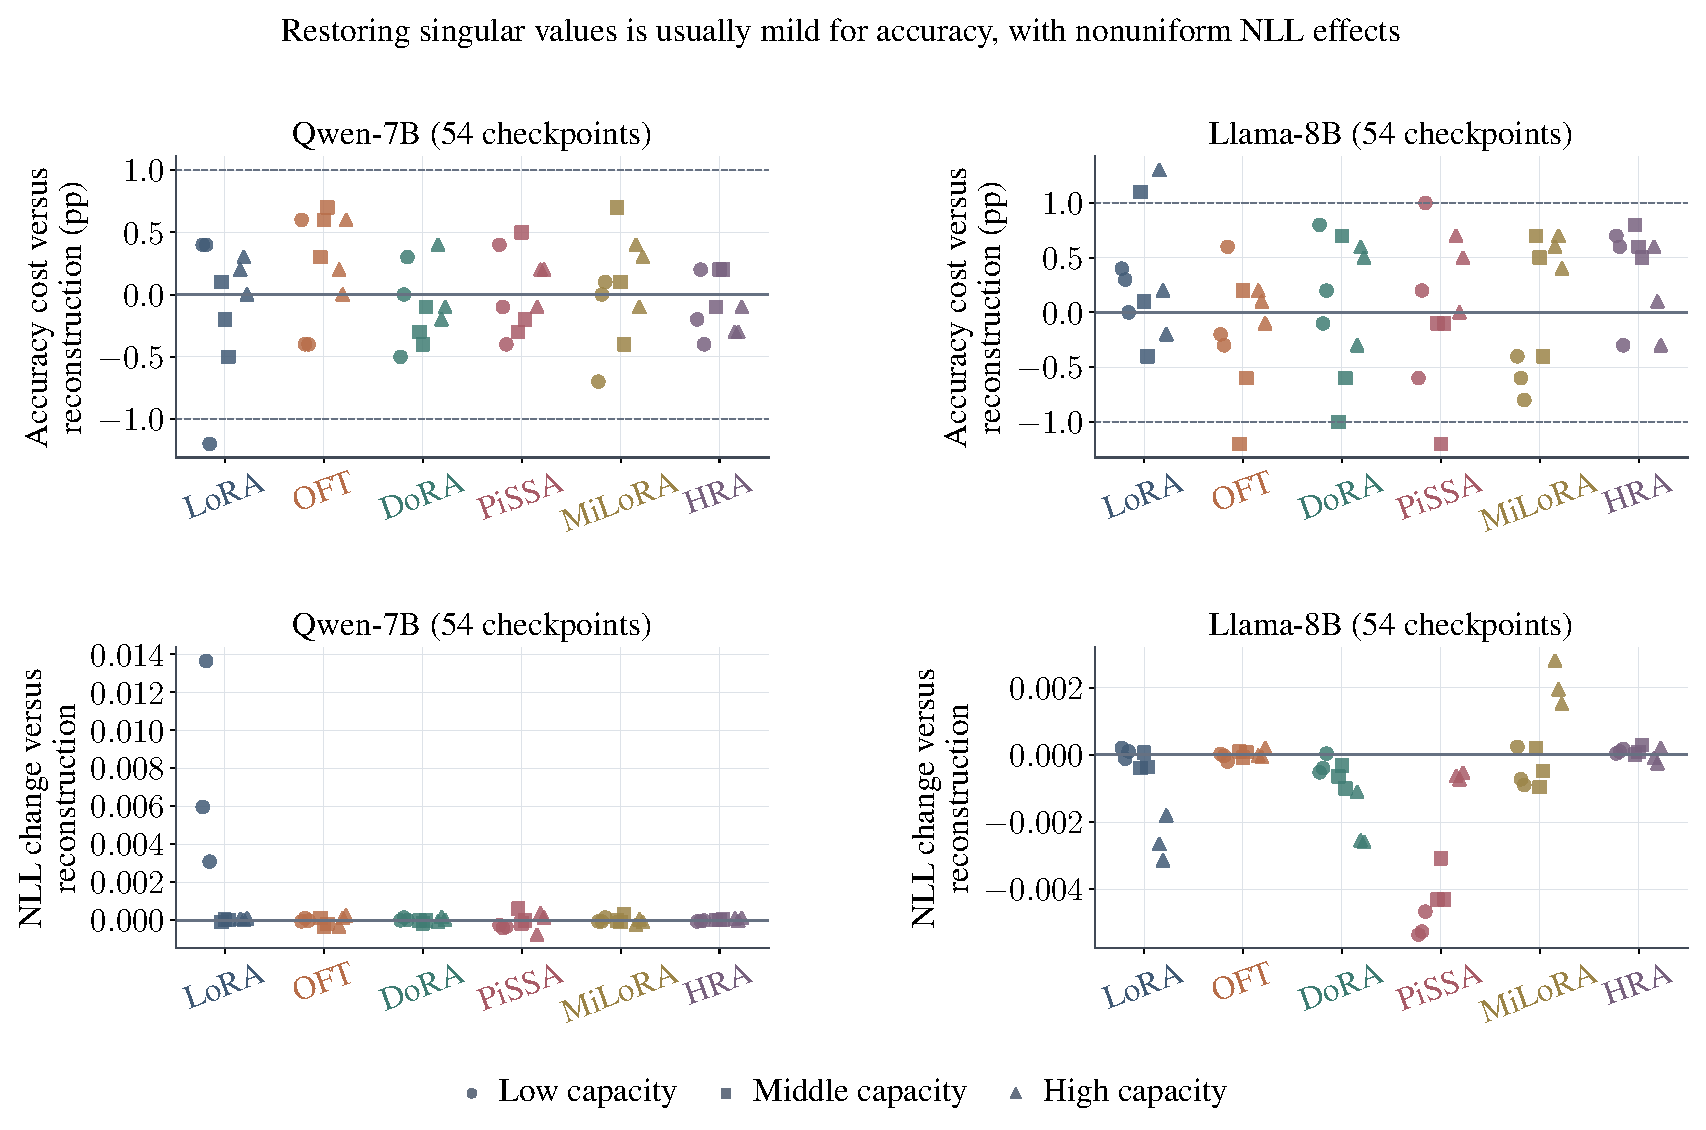
\includegraphics[width=\linewidth,height=.72\textheight,keepaspectratio]{figures/peft_app_03_value_restoration_controls.pdf}
\caption{Singular-value restoration across capacities and seeds. Trained, reconstructed and restored models are shown separately, extending the main accuracy comparison with reconstruction controls and retention measurements.}
\label{fig:complete-values}
\end{figure}
\begin{figure}[!htbp]\centering
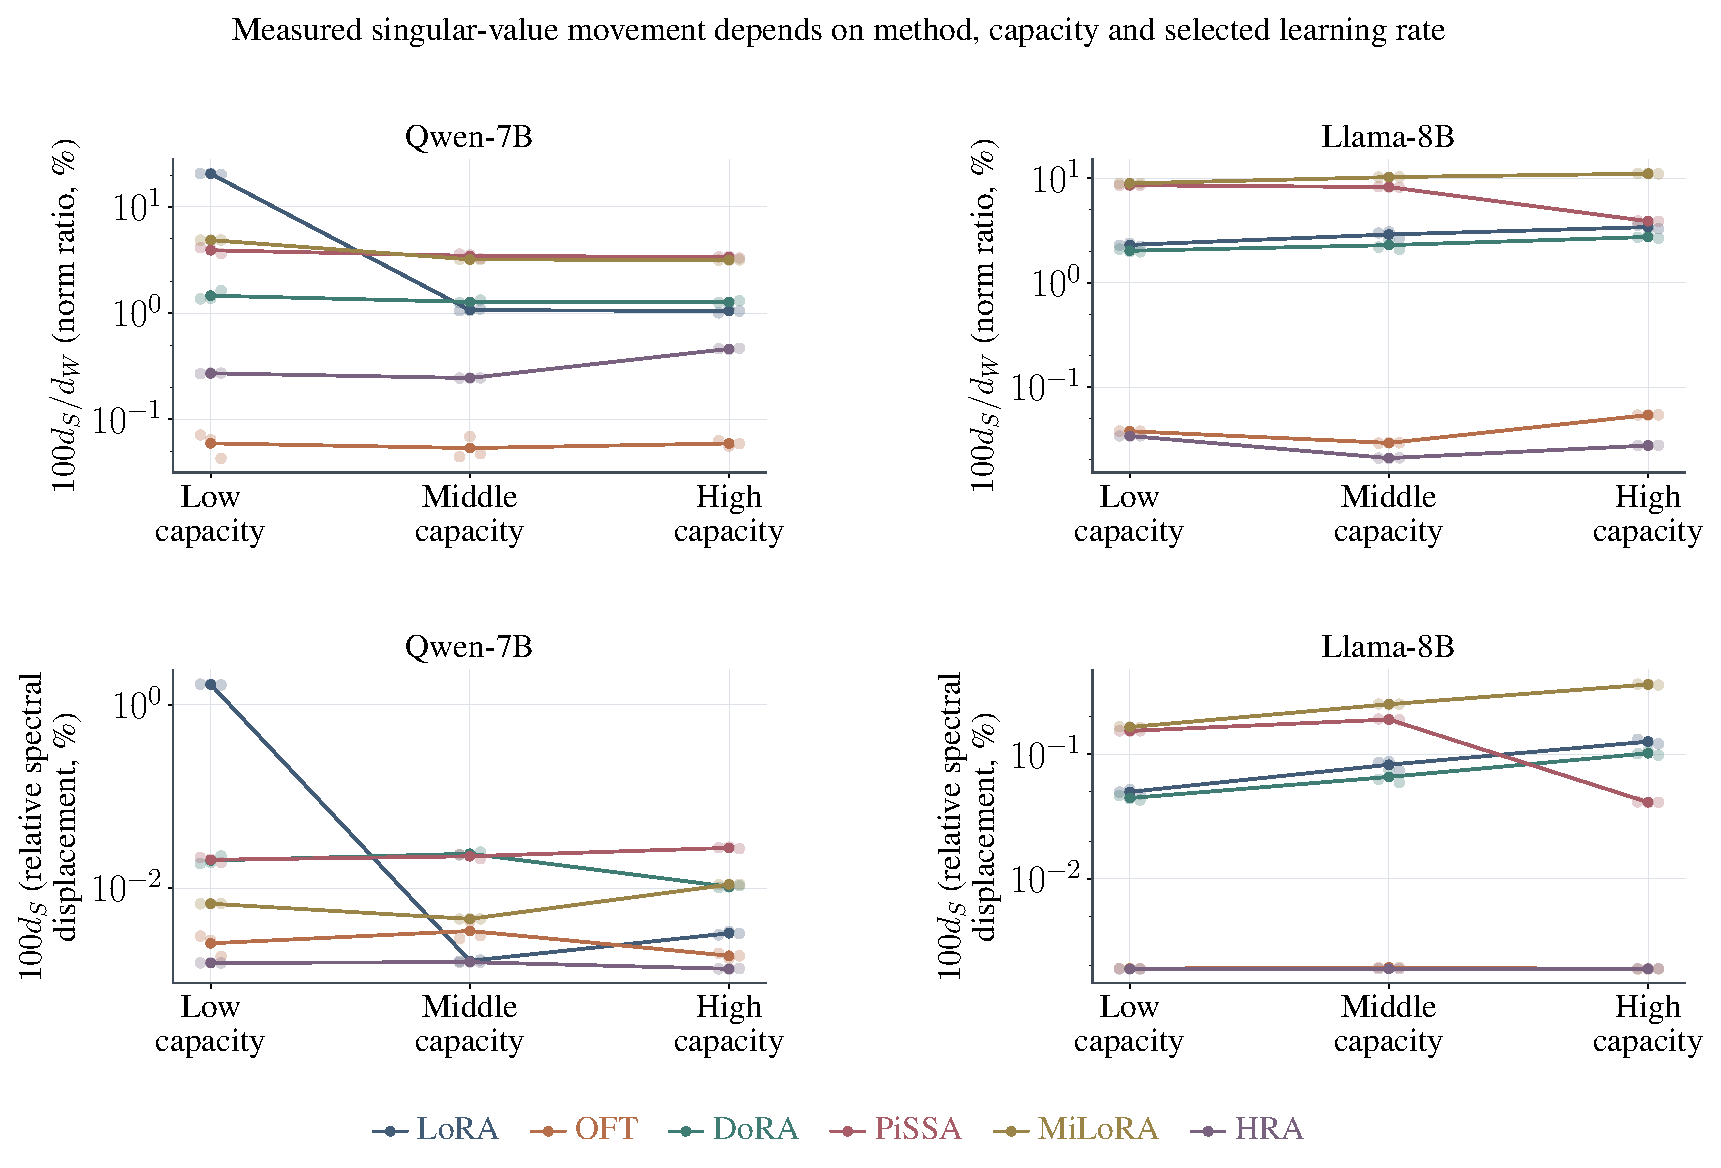
\includegraphics[width=\linewidth,height=.72\textheight,keepaspectratio]{figures/peft_app_07_spectral_displacement.pdf}
\caption{Measured weight and singular-value displacement across all six methods and both models at each selected capacity and LR. Ratios express spectral displacement relative to weight displacement.}
\end{figure}
\begin{figure}[!htbp]\centering
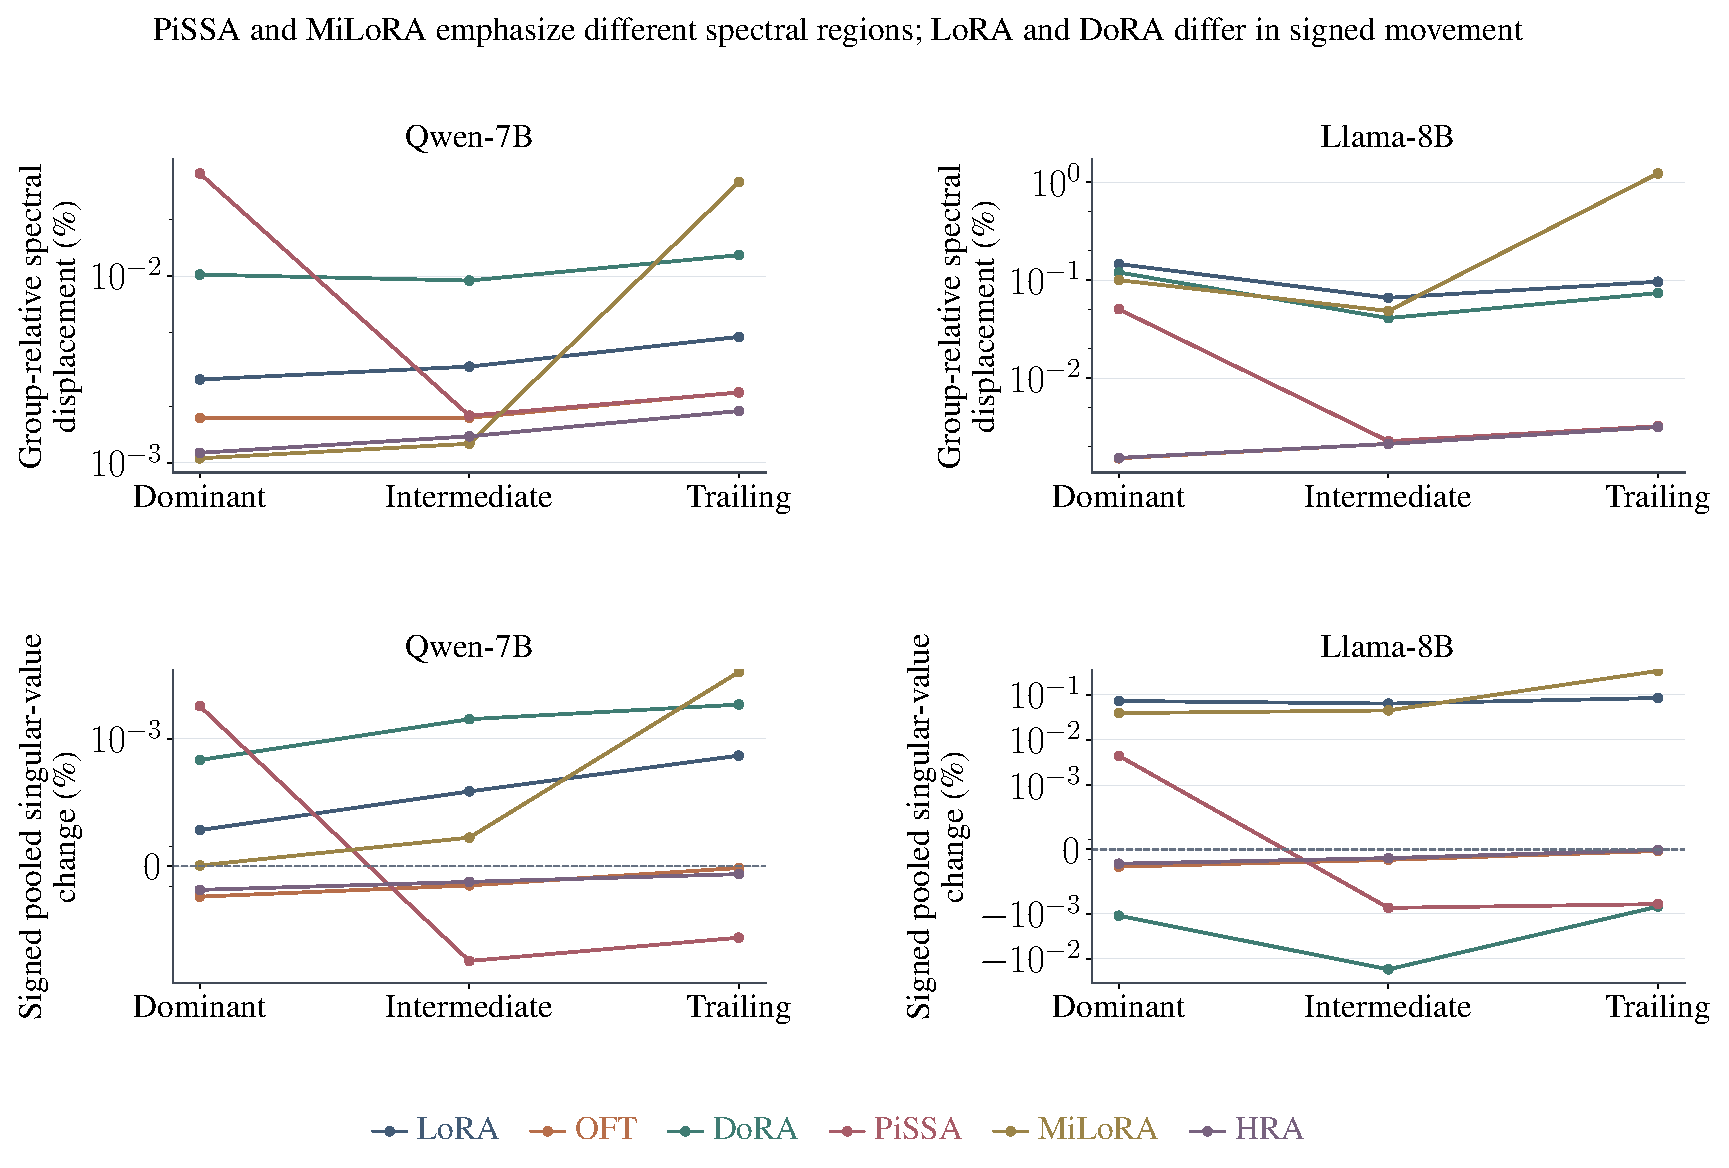
\includegraphics[width=\linewidth,height=.72\textheight,keepaspectratio]{figures/peft_app_08_bandwise_singular_values.pdf}
\caption{Singular-value changes across spectral components at largest capacity. PiSSA's displacement concentrates near the leading end, whereas MiLoRA's concentrates near the tail, consistent with their initialization choices. The pretrained reference and method colors are retained.}
\end{figure}



\Needspace{20\baselineskip}
\subsection{Hyperspherical energy and pairwise geometry}\label{app:hyperspherical}
We measure all adapted matrices in the largest-capacity intervention checkpoints, with 196 per Qwen model, 224 per Llama model and 80 per FLUX cat model. The 54 checkpoints and 9,000 matrix comparisons use the same selected LRs as the spectral and functional analyses. This tests whether the approximate geometric preservation observed for LoRA-family methods also extends to HE.

\paragraph{Definitions and aggregation.}
For stored weights $\bm W\in\mathbb R^{n\times d}$, rows represent output neurons. Let $\widehat{\bm w}_i=\bm w_i/\|\bm w_i\|_2$. Following \citet{liu2018mhe} and \citet{qiu2023oft}, we compute
\begin{equation*}
H(\bm W)=\sum_{i\ne j}\frac{1}{\|\widehat{\bm w}_i-\widehat{\bm w}_j\|_2},\qquad
\delta_H=\frac{|H(\bm W_*)-H(\bm W_0)|}{H(\bm W_0)}.
\end{equation*}
The sum covers every ordered distinct row pair. To measure pairwise changes without signed cancellation, we also compute
\begin{equation*}
\delta_C=\left[\frac{1}{n(n-1)}\sum_{i\ne j}
\left(\widehat{\bm w}_{*,i}^{\!\top}\widehat{\bm w}_{*,j}-\widehat{\bm w}_{0,i}^{\!\top}\widehat{\bm w}_{0,j}\right)^2\right]^{1/2}.
\end{equation*}
We average each metric equally over matrices within a checkpoint, then summarize training seeds. The absolute HE change is taken before matrix averaging. A common right-orthogonal transformation preserves row inner products and HE.

% Generated by analysis/integrate_hyperspherical.py; do not edit.
\begin{table}[!htbp]
\caption{Geometric preservation at largest selected capacities. Each checkpoint averages matrices equally, followed by the seed mean and sample SD. HE changes are in units of $10^{-4}\%$, and cosine changes are in units of $10^{-4}$.}
\label{tab:hyperspherical}
\begin{center}
\begin{tabular*}{\linewidth}{@{\extracolsep{\fill}}lccc@{}}\toprule
Method & Qwen2.5-7B & Llama-3.1-8B & FLUX-4B cat \\\midrule
\multicolumn{4}{l}{(a) Absolute relative HE change ($\times10^{-4}\%$)} \\
\textcolor{LoRAColor}{LoRA} & $14.8_{\pm 0.96}$ & $1.72_{\pm 0.17}$ & $0.281_{\pm 0.025}$ \\
\textcolor{OFTColor}{OFT} & $1.5_{\pm 0.2}$ & $0.0215_{\pm 0.0014}$ & $0.533_{\pm 0.065}$ \\
\textcolor{DoRAColor}{DoRA} & $80.3_{\pm 15}$ & $1.7_{\pm 0.069}$ & $0.714_{\pm 0.072}$ \\
\textcolor{PiSSAColor}{PiSSA} & $91.9_{\pm 4.6}$ & $1.53_{\pm 0.099}$ & $3.02_{\pm 0.24}$ \\
\textcolor{MiLoRAColor}{MiLoRA} & $1.35_{\pm 0.37}$ & $4.36_{\pm 0.17}$ & $0.987_{\pm 0.032}$ \\
\textcolor{HRAColor}{HRA} & $0.625_{\pm 0.12}$ & $0.0264_{\pm 0.0013}$ & $0.00804_{\pm 0.0008}$ \\
\midrule
\multicolumn{4}{l}{(b) Pairwise-cosine RMS change ($\times10^{-4}$)} \\
\textcolor{LoRAColor}{LoRA} & $0.906_{\pm 0.015}$ & $10.7_{\pm 0.15}$ & $2.51_{\pm 0.11}$ \\
\textcolor{OFTColor}{OFT} & $0.372_{\pm 0.00052}$ & $0.35_{\pm 2.3\times10^{-5}}$ & $0.48_{\pm 0.022}$ \\
\textcolor{DoRAColor}{DoRA} & $2.26_{\pm 0.034}$ & $10.6_{\pm 0.069}$ & $4.65_{\pm 0.08}$ \\
\textcolor{PiSSAColor}{PiSSA} & $5.33_{\pm 0.045}$ & $5.98_{\pm 0.011}$ & $17_{\pm 0.1}$ \\
\textcolor{MiLoRAColor}{MiLoRA} & $1.12_{\pm 0.0044}$ & $10.6_{\pm 0.1}$ & $4.11_{\pm 0.19}$ \\
\textcolor{HRAColor}{HRA} & $0.307_{\pm 0.001}$ & $0.35_{\pm 1.6\times10^{-5}}$ & $0.407_{\pm 5.9\times10^{-6}}$ \\
\bottomrule
\end{tabular*}
\end{center}
\end{table}


\begin{samepage}
\paragraph{Results.}
All checkpoint means of $\delta_H$ are below $0.01\%$, with maximum $\result{he_max_checkpoint_percent}\%$ (\Cref{tab:hyperspherical}). This supports approximate HE preservation across the selected LoRA-family methods as well as the orthogonal methods. The pairwise measure shows how closely individual neuron relationships are preserved alongside aggregate HE.
\par
\end{samepage}


\subsection{Component effects, interactions and task performance}
Restoring dominant components lowers general-text NLL at every capacity and gives the largest reduction among the three groups in 106/108 checkpoints. The exceptions to the largest reduction are Qwen DoRA r14/seed 73 and MiLoRA r28/seed 13. Dominant restoration remains strongest in every configuration mean, supporting the consistent forgetting response across language capacities.

\begin{figure}[!htbp]\centering
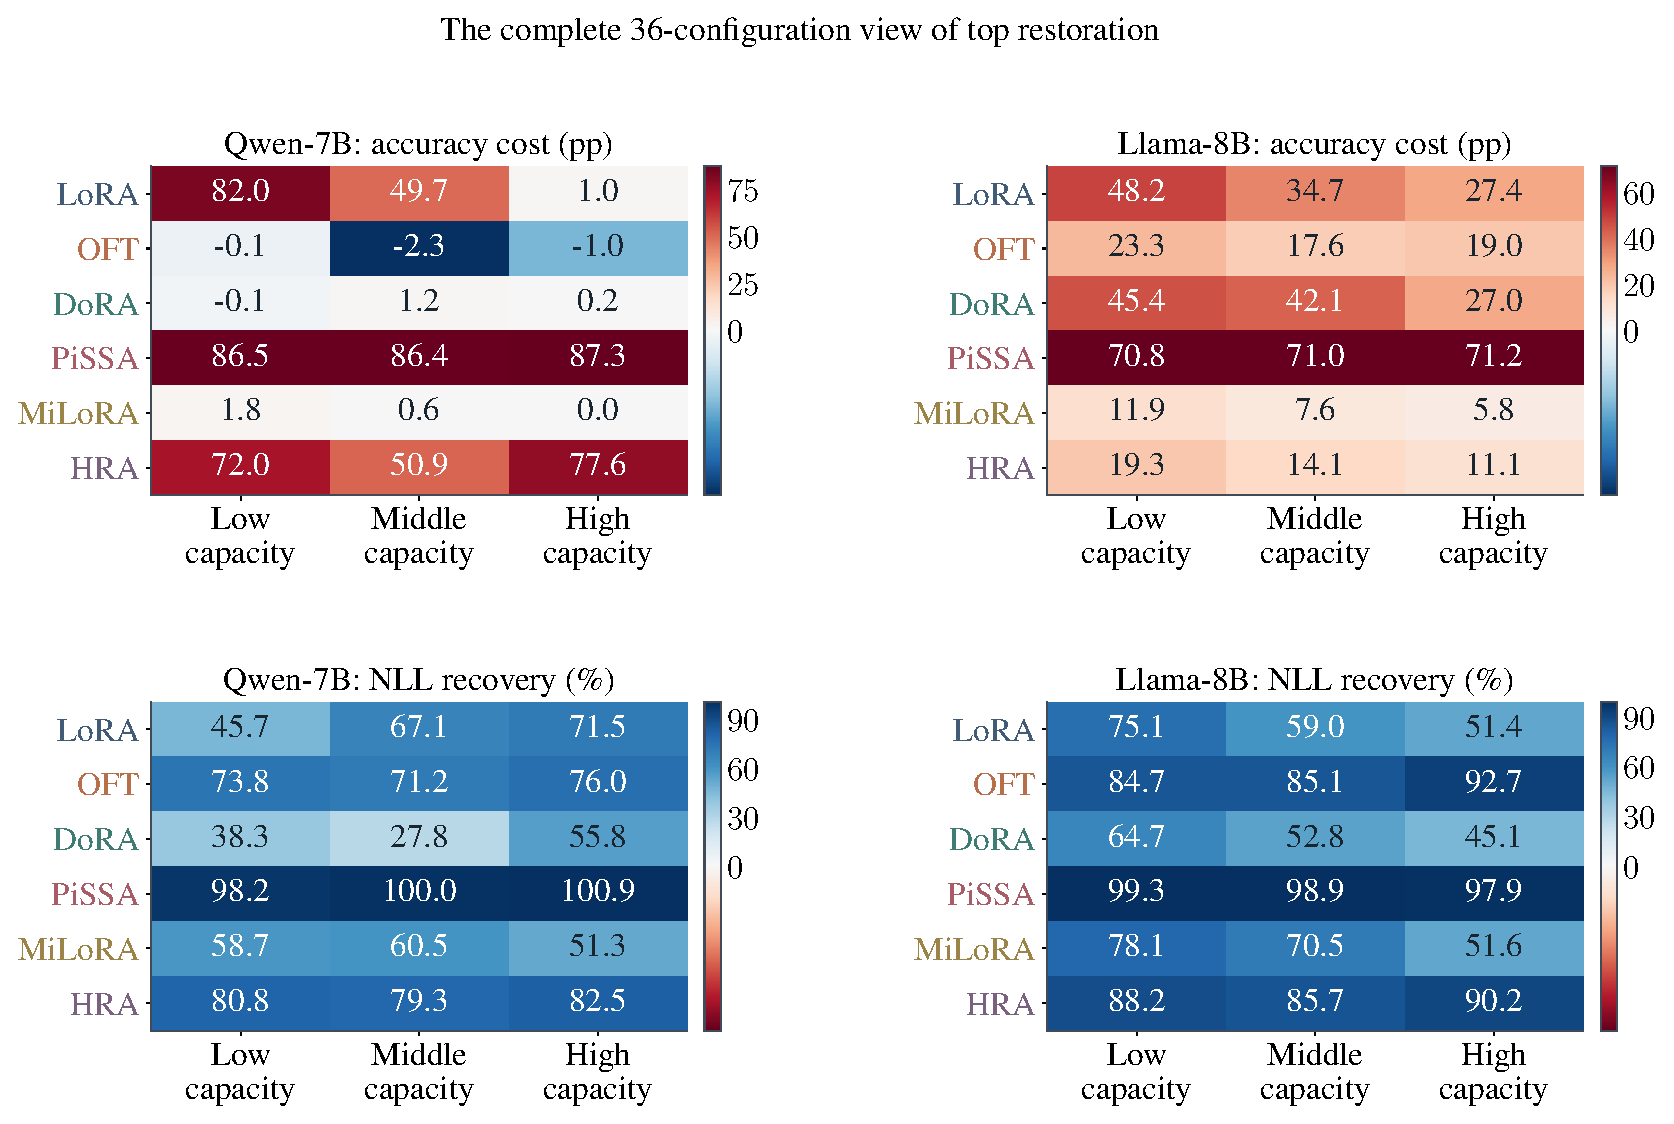
\includegraphics[width=\linewidth,height=.76\textheight,keepaspectratio]{figures/peft_app_02_all_configuration_top_resets.pdf}
\caption{Dominant-component restoration at every selected configuration and seed. The retention response persists across the grid, while task-accuracy responses vary. Recovery is normalized by each checkpoint's trained-model NLL increase.}
\end{figure}

For a set $A$ of adapted component groups, define
\begin{equation*}
\bm W(A)=\sum_{B\in A}\sum_{i\in B}s_{0,i}\bm u_{*,i}\bm v_{*,i}^{\!\top}
+\sum_{B\notin A}\sum_{i\in B}s_{0,i}\bm u_{0,i}\bm v_{0,i}^{\!\top}.
\end{equation*}
Its endpoints are the pretrained-component reconstruction and the full value-restored model. For general NLL $f(A)$, the effect of adapting group $B$ is $f(A\cup\{B\})-f(A)$. We evaluate it under all four combinations of pretrained or adapted components in the other groups. Adapting dominant components increases NLL in every combination across all 108 checkpoints. Intermediate and trailing effects change sign across combinations in 38 and 42 checkpoints, using a $10^{-4}$ tolerance. Thus, the dominant-component forgetting response persists as the other components change.

All 36 configurations include evaluations of every component combination for all three seeds.
\begin{figure}[!htbp]\centering
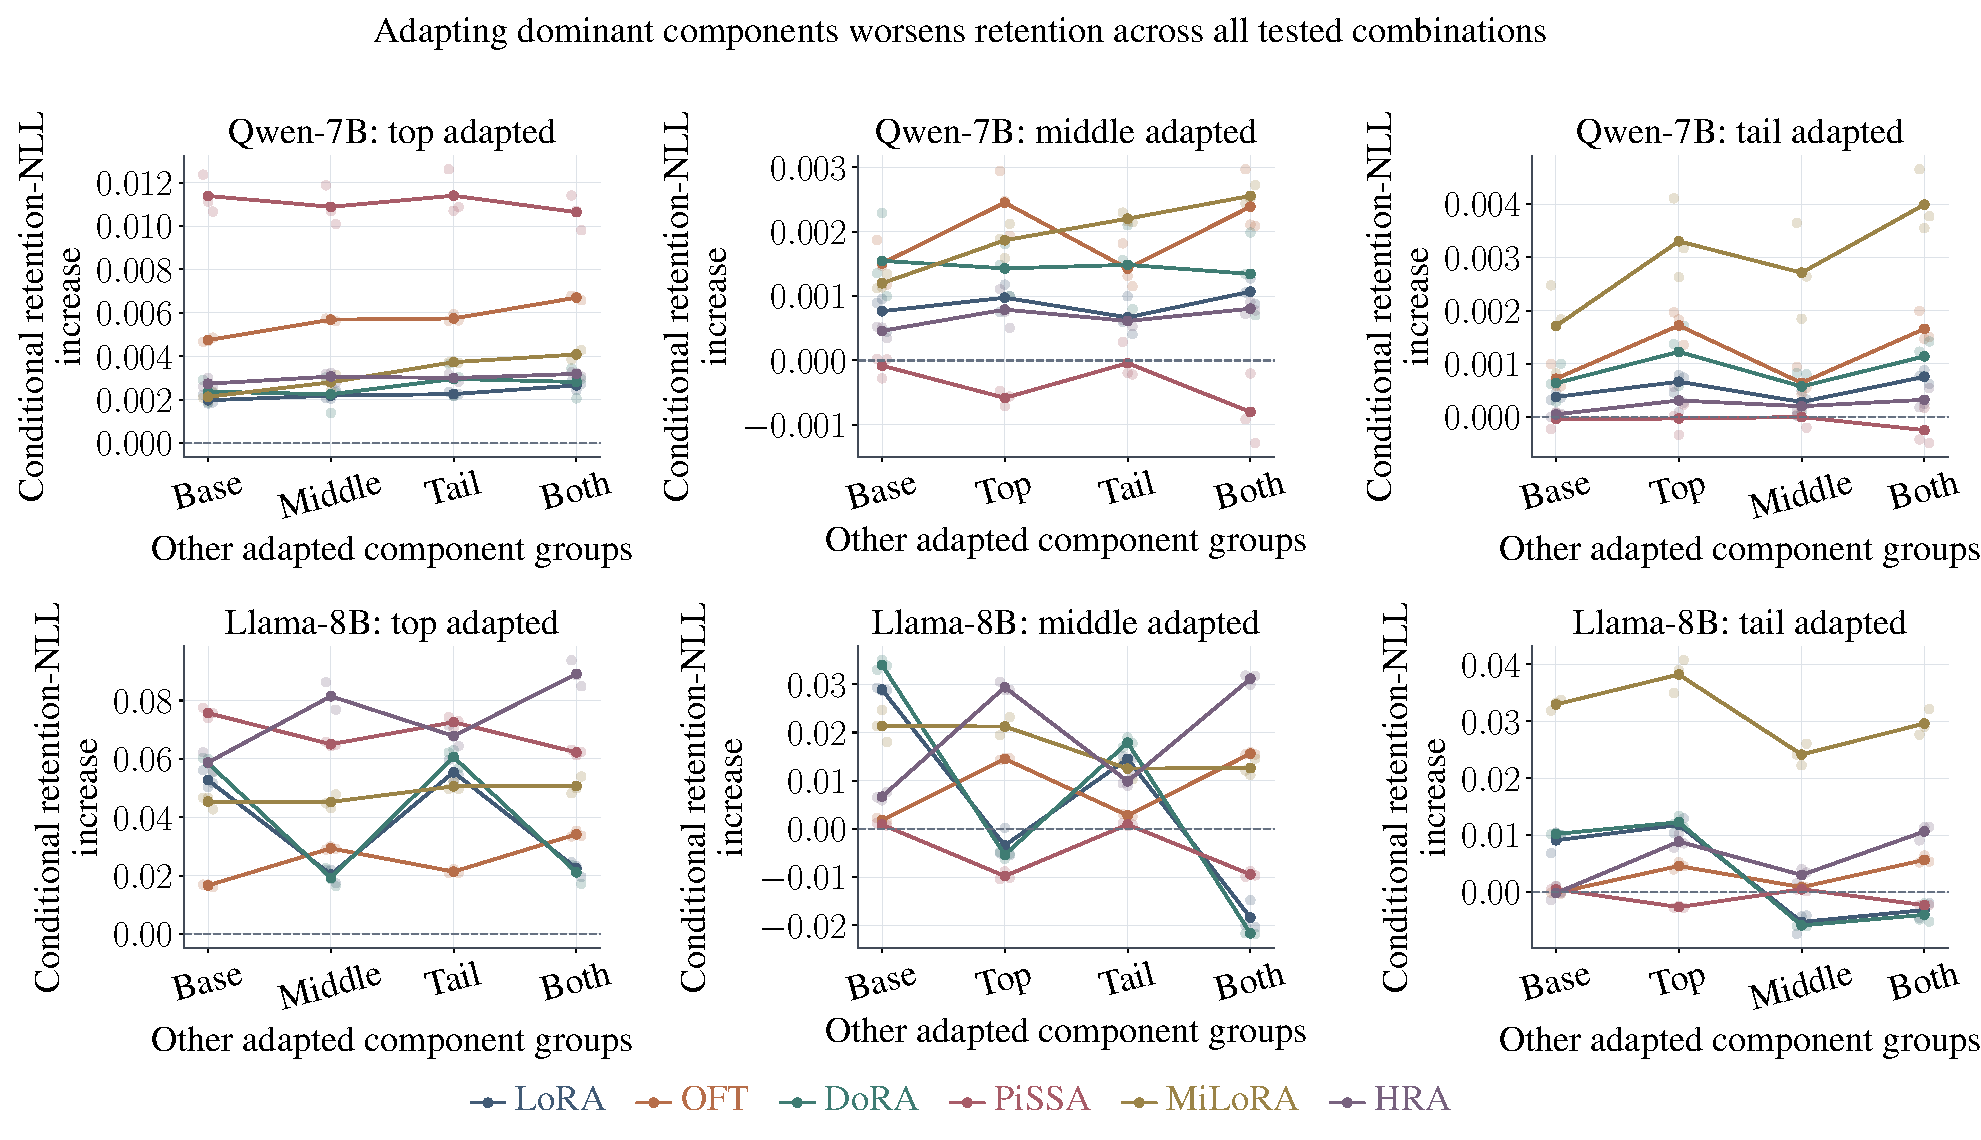
\includegraphics[width=\linewidth,height=.75\textheight,keepaspectratio]{figures/peft_app_04_conditional_band_effects.pdf}
\caption{Effects of adapting each component group under all combinations of the other groups. Dominant-component adaptation consistently increases general NLL, while intermediate and trailing effects can change sign. Both NLL evaluations agree on the dominant-component direction.}
\end{figure}
\begin{figure}[t]\centering
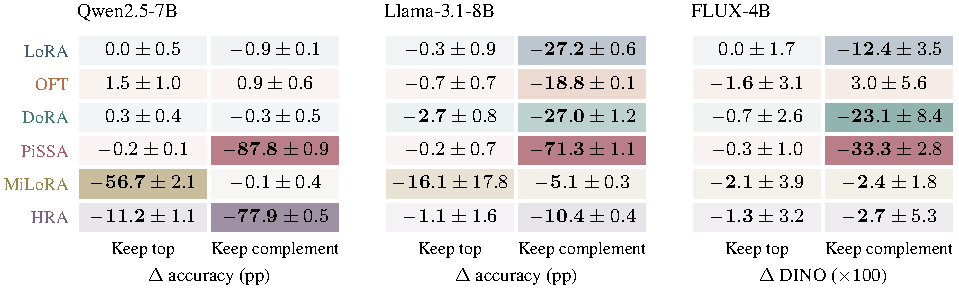
\includegraphics[width=\linewidth]{figures/peft_keep_reset.pdf}
\caption{Task performance when retaining only some adapted components. Cells show mean $\pm$ SD changes from $\bm W_R$ (all singular values restored) at the largest capacities. Columns retain the adapted dominant components alone or the intermediate and trailing components together. Bold means mark losses exceeding 1 pp for LLMs or 1 DINO$\times100$ unit for FLUX.}
\label{fig:component-sufficiency}
\end{figure}

\paragraph{Task performance across selected capacities.}
\Cref{tab:capacity-sufficiency} extends the largest-capacity comparison in \Cref{fig:component-sufficiency}. Qwen LoRA retains task performance with dominant components alone at small capacity, with neither component set alone at medium capacity, and with either set alone at large capacity. Llama LoRA's outcomes also vary across capacities and seeds. PiSSA retains the dominant-only pattern at every language capacity, supporting its consistent concentration of task gains in dominant components. The other methods illustrate the setting-dependent component contributions described in the main text, alongside the consistent forgetting response.
\begin{table}[!htbp]
\caption{Task sufficiency across all selected language capacities. Entries count seeds with accuracy loss $\leq1$ pp relative to full value restoration, out of three seeds per configuration. Top and complement retain those adapted components on a pretrained background. Tables~\ref{tab:peft-spectrum-qwen} and~\ref{tab:peft-spectrum-llama} give capacities and selected LRs.}
\label{tab:capacity-sufficiency}
\begin{center}
\setlength{\tabcolsep}{4pt}
\begin{tabular*}{\linewidth}{@{\extracolsep{\fill}}llcccccc@{}}\toprule
Model & Method & \multicolumn{2}{c}{Small} & \multicolumn{2}{c}{Medium} & \multicolumn{2}{c}{Large}\\
\cmidrule(lr){3-4}\cmidrule(lr){5-6}\cmidrule(l){7-8}
& & Top & Complement & Top & Complement & Top & Complement\\\midrule
Qwen2.5-7B & \textcolor{LoRAColor}{LoRA} & \result{rev_capacity_qwen_lora_7_top}/\result{rev_capacity_qwen_lora_7_valid} & \result{rev_capacity_qwen_lora_7_complement}/\result{rev_capacity_qwen_lora_7_valid} & \result{rev_capacity_qwen_lora_14_top}/\result{rev_capacity_qwen_lora_14_valid} & \result{rev_capacity_qwen_lora_14_complement}/\result{rev_capacity_qwen_lora_14_valid} & \result{rev_capacity_qwen_lora_28_top}/\result{rev_capacity_qwen_lora_28_valid} & \result{rev_capacity_qwen_lora_28_complement}/\result{rev_capacity_qwen_lora_28_valid}\\
 & \textcolor{OFTColor}{OFT} & \result{rev_capacity_qwen_oft_32_top}/\result{rev_capacity_qwen_oft_32_valid} & \result{rev_capacity_qwen_oft_32_complement}/\result{rev_capacity_qwen_oft_32_valid} & \result{rev_capacity_qwen_oft_64_top}/\result{rev_capacity_qwen_oft_64_valid} & \result{rev_capacity_qwen_oft_64_complement}/\result{rev_capacity_qwen_oft_64_valid} & \result{rev_capacity_qwen_oft_128_top}/\result{rev_capacity_qwen_oft_128_valid} & \result{rev_capacity_qwen_oft_128_complement}/\result{rev_capacity_qwen_oft_128_valid}\\
 & \textcolor{DoRAColor}{DoRA} & \result{rev_capacity_qwen_dora_7_top}/\result{rev_capacity_qwen_dora_7_valid} & \result{rev_capacity_qwen_dora_7_complement}/\result{rev_capacity_qwen_dora_7_valid} & \result{rev_capacity_qwen_dora_14_top}/\result{rev_capacity_qwen_dora_14_valid} & \result{rev_capacity_qwen_dora_14_complement}/\result{rev_capacity_qwen_dora_14_valid} & \result{rev_capacity_qwen_dora_28_top}/\result{rev_capacity_qwen_dora_28_valid} & \result{rev_capacity_qwen_dora_28_complement}/\result{rev_capacity_qwen_dora_28_valid}\\
 & \textcolor{PiSSAColor}{PiSSA} & \result{rev_capacity_qwen_pissa_7_top}/\result{rev_capacity_qwen_pissa_7_valid} & \result{rev_capacity_qwen_pissa_7_complement}/\result{rev_capacity_qwen_pissa_7_valid} & \result{rev_capacity_qwen_pissa_14_top}/\result{rev_capacity_qwen_pissa_14_valid} & \result{rev_capacity_qwen_pissa_14_complement}/\result{rev_capacity_qwen_pissa_14_valid} & \result{rev_capacity_qwen_pissa_28_top}/\result{rev_capacity_qwen_pissa_28_valid} & \result{rev_capacity_qwen_pissa_28_complement}/\result{rev_capacity_qwen_pissa_28_valid}\\
 & \textcolor{MiLoRAColor}{MiLoRA} & \result{rev_capacity_qwen_milora_7_top}/\result{rev_capacity_qwen_milora_7_valid} & \result{rev_capacity_qwen_milora_7_complement}/\result{rev_capacity_qwen_milora_7_valid} & \result{rev_capacity_qwen_milora_14_top}/\result{rev_capacity_qwen_milora_14_valid} & \result{rev_capacity_qwen_milora_14_complement}/\result{rev_capacity_qwen_milora_14_valid} & \result{rev_capacity_qwen_milora_28_top}/\result{rev_capacity_qwen_milora_28_valid} & \result{rev_capacity_qwen_milora_28_complement}/\result{rev_capacity_qwen_milora_28_valid}\\
 & \textcolor{HRAColor}{HRA} & \result{rev_capacity_qwen_hra_16_top}/\result{rev_capacity_qwen_hra_16_valid} & \result{rev_capacity_qwen_hra_16_complement}/\result{rev_capacity_qwen_hra_16_valid} & \result{rev_capacity_qwen_hra_32_top}/\result{rev_capacity_qwen_hra_32_valid} & \result{rev_capacity_qwen_hra_32_complement}/\result{rev_capacity_qwen_hra_32_valid} & \result{rev_capacity_qwen_hra_64_top}/\result{rev_capacity_qwen_hra_64_valid} & \result{rev_capacity_qwen_hra_64_complement}/\result{rev_capacity_qwen_hra_64_valid}\\
\midrule
Llama-3.1-8B & \textcolor{LoRAColor}{LoRA} & \result{rev_capacity_llama_lora_7_top}/\result{rev_capacity_llama_lora_7_valid} & \result{rev_capacity_llama_lora_7_complement}/\result{rev_capacity_llama_lora_7_valid} & \result{rev_capacity_llama_lora_15_top}/\result{rev_capacity_llama_lora_15_valid} & \result{rev_capacity_llama_lora_15_complement}/\result{rev_capacity_llama_lora_15_valid} & \result{rev_capacity_llama_lora_30_top}/\result{rev_capacity_llama_lora_30_valid} & \result{rev_capacity_llama_lora_30_complement}/\result{rev_capacity_llama_lora_30_valid}\\
 & \textcolor{OFTColor}{OFT} & \result{rev_capacity_llama_oft_32_top}/\result{rev_capacity_llama_oft_32_valid} & \result{rev_capacity_llama_oft_32_complement}/\result{rev_capacity_llama_oft_32_valid} & \result{rev_capacity_llama_oft_64_top}/\result{rev_capacity_llama_oft_64_valid} & \result{rev_capacity_llama_oft_64_complement}/\result{rev_capacity_llama_oft_64_valid} & \result{rev_capacity_llama_oft_128_top}/\result{rev_capacity_llama_oft_128_valid} & \result{rev_capacity_llama_oft_128_complement}/\result{rev_capacity_llama_oft_128_valid}\\
 & \textcolor{DoRAColor}{DoRA} & \result{rev_capacity_llama_dora_7_top}/\result{rev_capacity_llama_dora_7_valid} & \result{rev_capacity_llama_dora_7_complement}/\result{rev_capacity_llama_dora_7_valid} & \result{rev_capacity_llama_dora_15_top}/\result{rev_capacity_llama_dora_15_valid} & \result{rev_capacity_llama_dora_15_complement}/\result{rev_capacity_llama_dora_15_valid} & \result{rev_capacity_llama_dora_30_top}/\result{rev_capacity_llama_dora_30_valid} & \result{rev_capacity_llama_dora_30_complement}/\result{rev_capacity_llama_dora_30_valid}\\
 & \textcolor{PiSSAColor}{PiSSA} & \result{rev_capacity_llama_pissa_7_top}/\result{rev_capacity_llama_pissa_7_valid} & \result{rev_capacity_llama_pissa_7_complement}/\result{rev_capacity_llama_pissa_7_valid} & \result{rev_capacity_llama_pissa_15_top}/\result{rev_capacity_llama_pissa_15_valid} & \result{rev_capacity_llama_pissa_15_complement}/\result{rev_capacity_llama_pissa_15_valid} & \result{rev_capacity_llama_pissa_30_top}/\result{rev_capacity_llama_pissa_30_valid} & \result{rev_capacity_llama_pissa_30_complement}/\result{rev_capacity_llama_pissa_30_valid}\\
 & \textcolor{MiLoRAColor}{MiLoRA} & \result{rev_capacity_llama_milora_7_top}/\result{rev_capacity_llama_milora_7_valid} & \result{rev_capacity_llama_milora_7_complement}/\result{rev_capacity_llama_milora_7_valid} & \result{rev_capacity_llama_milora_15_top}/\result{rev_capacity_llama_milora_15_valid} & \result{rev_capacity_llama_milora_15_complement}/\result{rev_capacity_llama_milora_15_valid} & \result{rev_capacity_llama_milora_30_top}/\result{rev_capacity_llama_milora_30_valid} & \result{rev_capacity_llama_milora_30_complement}/\result{rev_capacity_llama_milora_30_valid}\\
 & \textcolor{HRAColor}{HRA} & \result{rev_capacity_llama_hra_16_top}/\result{rev_capacity_llama_hra_16_valid} & \result{rev_capacity_llama_hra_16_complement}/\result{rev_capacity_llama_hra_16_valid} & \result{rev_capacity_llama_hra_32_top}/\result{rev_capacity_llama_hra_32_valid} & \result{rev_capacity_llama_hra_32_complement}/\result{rev_capacity_llama_hra_32_valid} & \result{rev_capacity_llama_hra_64_top}/\result{rev_capacity_llama_hra_64_valid} & \result{rev_capacity_llama_hra_64_complement}/\result{rev_capacity_llama_hra_64_valid}\\
\bottomrule\end{tabular*}
\end{center}
\end{table}


\FloatBarrier
\subsection{Consistency of the dominant-component response}\label{app:component-consistency}
The comparison covers 42 selected configurations and 126 checkpoints across all six methods, all tested language capacities and the largest FLUX budget for each method. Restoring dominant components gives the largest mean reduction in general-text NLL or general-image drift in all 42 configurations and a larger reduction than restoring either intermediate or trailing components in 123/126 checkpoints. These counts support the recurring dominant-component forgetting response across models and tasks.

\paragraph{Consistency with smaller edits.}
We measure edit norm as the square root of the summed squared Frobenius changes from trained weights across all adapted matrices, using the stored weights. We select cases where restoring intermediate or trailing components produces a larger edit norm than restoring dominant components. Configuration comparisons use seed means of norms and forgetting reductions. Dominant restoration still gives the largest mean forgetting reduction among all three restorations in 17/17 eligible configurations, comprising 8 Qwen, 6 Llama and 3 FLUX configurations. At the checkpoint level, the count is 48/51, with 22/24 for Qwen, 18/18 for Llama and 8/9 for FLUX. Each configuration or checkpoint is counted once, including when both alternatives have larger norms. Requiring both alternatives to have larger norms gives 4/4 configurations and 10/12 checkpoints. The eligible cases involve LoRA, DoRA and MiLoRA. These counts show that the dominant-component advantage can persist with smaller edits, so edit magnitude alone does not determine the ordering of forgetting reductions.


\FloatBarrier
\subsection{Native OFT orthogonality and polar projection}\label{app:native-orthogonality}
OFTv2 approximates the Cayley inverse with a truncated Neumann series \citep{qiu2025oftv2}. We measure $\|\bm R\bm R^{\!\top}-\bm I\|_{\mathrm{F}}$, its maximum absolute entry, and $\|\bm R-\widehat{\bm R}\|_{\mathrm{F}}/\|\bm R\|_{\mathrm{F}}$, where $\widehat{\bm R}$ is the polar factor \citep{higham1986polar}. The relative distance expresses the deviation from orthogonality on a scale normalized by the transform norm. These diagnostics cover 21 checkpoints each for Qwen and Llama, and 33 for FLUX. The maximum native-to-polar distances are about 0.154\%, 0.094\% and 11.0\%, respectively (\Cref{tab:peft-orthogonality}). Task and retention evaluations use native transforms. Polar projection measures their deviation from an exact orthogonal transform, clarifying the numerical precision of the geometric-preservation comparison.

\begin{table}[!htbp]\caption{Native OFT-transform diagnostics. Maxima are taken over all matrices and checkpoints in each row. Frobenius and entrywise maxima describe different norms.}\label{tab:peft-orthogonality}
\begin{center}
\begin{tabular}{lrrrr}\toprule Model & Checkpoints & Max. $\|\bm R\bm R^{\!\top}-\bm I\|_{\mathrm{F}}$ & Max. entry & Max. polar residual\\\midrule
FLUX-4B & 33 & $8.04$ & $0.136$ & $0.11$\\
Llama-8B & 21 & $0.118$ & $0.00528$ & $0.000936$\\
Qwen-7B & 21 & $0.42$ & $0.0233$ & $0.00154$\\
\bottomrule\end{tabular}
\end{center}
\end{table}

